\documentclass[11pt]{article}
\usepackage{amsmath, amsthm, amssymb, pdfpages} 
\usepackage{fullpage}
\usepackage{hyperref}
\usepackage{graphicx}
\usepackage[capitalize]{cleveref}
\usepackage{appendix}

% next three for UTF8 to work (for non-ASCII names to work without awkward codes)
\usepackage[T1]{fontenc}
\usepackage{textcomp}
\usepackage[utf8]{inputenc}

% import biblatex with prefered settings
% reuse code and library from LIGERA paper in the same repository
% loads biblatex with all the nice standard options that John determined some time ago!
% this version uses a ``Harvard'' style (first author last name, year in parentheses).
% also loads xpatch

% biblatex
% harvard style
\usepackage[style=authoryear,natbib,maxcitenames=2,doi=true,isbn=false,url=false,backend=bibtex]{biblatex}
% numeric style
%% \usepackage[style=numeric-comp,sorting=none,giveninits=true,
%%                      doi=false,isbn=false,url=false,backend=bibtex]{biblatex}
% remove "In: " before journal title
\renewbibmacro{in:}{}
% remove language
\AtEveryBibitem{\clearlist{language}}
% remove month
\AtEveryBibitem{\clearfield{month}}
% and also notes
\AtEveryBibitem{\clearfield{note}}
% remove dots between volume and issue
\usepackage{xpatch}
\xpatchbibmacro{volume+number+eid}{%
  \setunit*{\adddot}%
}{%
}{}{}
% put issue in parentheses
\DeclareFieldFormat[article]{number}{\mkbibparens{#1}}


\bibliography{zotero} % biblatex wants this in the preamble...

% copied from PCA-GWAS paper
\newcommand{\rmsd}{\text{SRMSD}_p}
\newcommand{\auc}{\text{AUC}_\text{PR}}

\usepackage[noT]{kinshipsymbols}
% % copy of \Fst from package `kinshipsymbols`

% some more definitions
\newcommand{\kinMat}{%
  \ensuremath{%
    \mathbf{\Phi}
  }%
  \xspace%
}%
\newcommand{\kinMatEstNamed}[1]{%
  \ensuremath{%
    \mathbf{\hat{\Phi}}^\text{#1}
  }%
  \xspace%
}%
\newcommand{\kinMatStdLim}{%
  \kinMatEstNamed{std-lim}
}%
\newcommand{\kinMatWGLim}{%
  \kinMatEstNamed{WG-lim}
}%

% % for theorems!
% \usepackage{amsthm}
% %\newtheorem{thm}{Theorem}[section]
% \newtheorem*{thm}{Theorem}
% %\newtheorem{lem}[thm]{Lemma}
% \newtheorem*{lem}{Lemma}
% % \newtheorem{lemma}[theorem]{Lemma}

% % double line spacing (PLoS wants this)
% \usepackage{setspace}
% \doublespacing
% spacing smaller than double
\renewcommand{\baselinestretch}{1.2}

% cool automatic supplemental figures/tables!
% http://bytesizebio.net/2013/03/11/adding-supplementary-tables-and-figures-in-latex/
% with some additions
\newcommand{\beginsupplement}{%
  \setcounter{table}{0}
  \renewcommand{\thetable}{S\arabic{table}}%
  \setcounter{figure}{0}
  \renewcommand{\thefigure}{S\arabic{figure}}%
  \setcounter{section}{0}
  \renewcommand{\thesection}{S\arabic{section}}%
  \setcounter{equation}{0}
  \renewcommand{\theequation}{S\arabic{equation}}%
  \setcounter{page}{1}
  \renewcommand{\thepage}{S\arabic{page}}%
}


\title{\Large \textbf{Fixed and mixed-effect genetic association models are robust to common population kinship estimation biases}}
\author{Zhuoran Hou$^1$, Alejandro Ochoa$^{1,2,*}$}
\date{}

\begin{document}
\maketitle

\noindent
$^1$ Department of Biostatistics and Bioinformatics, Duke University, Durham, NC 27705, USA \\
$^2$ Duke Center for Statistical Genetics and Genomics, Duke University, Durham, NC 27705, USA \\
$^*$ Corresponding author: \texttt{alejandro.ochoa@duke.edu}


\begin{abstract}
  Genetic association studies for structured populations model the correlation structure between individuals, most often using population kinship matrices.
  The two most common association models, Principal Components Analysis (PCA) association and the Linear Mixed-effects Model (LMM), are expressed in terms of kinship matrices.
  However, the most common kinship estimators can have severe biases that were only recently characterized.
  The goal of this work is to characterize the effect of these kinship biases on genetic association.
  We employed a large simulated admixed family and data from the 1000 Genomes Project, both with simulated traits, to evaluate the performance of each of PCA and LMM when a variety of kinship matrices is used.
  We tested several common kinship estimators, and in the simulated admixed family we also included the true kinship matrix and the the theoretical limits of the biased estimators (as the number of loci approaches infinity).
  Remarkably, we find negligible differences in association statistics and overall performance between all kinship matrices tested.
  Our empirical observations led us to the hypothesis that the association tests are invariant to whether the true kinship matrix or two of the biased limits are employed.
  We prove, using linear algebra, that our hypothesis holds exactly for LMM and approximately for PCA.
  Our constructive proof shows that both biased kinship matrices result in regression covariates (PCs in PCA, random effects in LMM) whose biases are compensated for by fitting the intercept, suggesting that only models with this precise arrangement will be robust to these kinship biases.
\end{abstract}

\clearpage

\section{Introduction}

% direct copy from Part II
Kinship is utilized in principal components analyses and linear-mixed effects models to correct for structure in Genome-Wide Association Studies (GWAS) \citep{xie_combining_1998,yu_unified_2006, aulchenko_genomewide_2007, price_principal_2006, astle_population_2009,kang_efficient_2008, kang_variance_2010, yang_gcta:_2011, zhou_genome-wide_2012, yang_advantages_2014, loh_efficient_2015, sul_population_2018}.
The most commonly-used kinship estimator \citep{price_principal_2006, astle_population_2009, rakovski_kinship-based_2009, thornton_roadtrips:_2010, yang_common_2010, yang_gcta:_2011, zhou_genome-wide_2012, speed_improved_2012, yang_advantages_2014, speed_relatedness_2015, loh_efficient_2015, wang_efficient_2017, sul_population_2018} was recently determined to have a complex bias \citep{weir_unified_2017, ochoa_estimating_2021}.

WG has a simpler, uniform bias \citep{weir_unified_2017, ochoa_estimating_2021}.

popkin is unbiased  \citep{ochoa_estimating_2021}.

We demonstrate our findings using an admixed family simulation \citep{yao_limitations_2022} as well as real genotypes from the 1000 Genomes project \citep{the_1000_genomes_project_consortium_map_2010, 1000_genomes_project_consortium_integrated_2012, fairley_international_2020}.


\section{Methods}

\subsection{Genetic model}

The following genetic model justifies the use of kinship matrices in association studies, and is the basis of all kinship estimation bias calculations that our theoretical work depends upon.

Suppose there are $m$ biallelic loci and $n$ diploid individuals.
The genotype $\xij \in \{0,1,2\}$ at a locus $i$ of individual $j$ is encoded as the number of reference alleles, for a preselected but otherwise arbitrary reference allele per locus.
These genotypes can be treated as random variables structured according to relatedness.
If \kt is the kinship coefficient of two individuals $j$ and $k$, and \pit is the ancestral allele frequency at locus $i$, then under the kinship model \citep{ochoa_estimating_2021} the expectation and covariance are given by
\begin{align*}
  \E[\mathbf{X}]
  =
    2 \mathbf{p} \mathbf{1}^\intercal
  ,
  \quad\quad
  \Cov(\mathbf{x}_i)
  =
    4 \pit (1-\pit) \kinMat
    ,
\end{align*}
where $\mathbf{x}_i$ is the length-$n$ column vector of genotypes at locus $i$, $\mathbf{X} = (\mathbf{x}_i^\intercal)$ is the complete $m \times n$ genotype matrix, $\kinMat = (\kt)$ is the $n \times n$ kinship matrix, $\mathbf{p} = (\pit)$ is a length-$m$ column vector of ancestral allele frequencies, $\mathbf{1} = (1)$ is a length-$n$ column vector where every element is 1, and the $\intercal$ superscript denotes matrix transposition.
Both kinship ($\kinMat$) and ancestral allele frequencies ($\mathbf{p}$) are parameters that depend on the choice of ancestral population, for which the Most Recent Common Ancestor (MRCA) population is the most sensible choice \citep{ochoa_estimating_2021}.
In this work, to simplify notation, we omit cumbersome notation that marks this dependence of parameters on the choice of ancestral population, nor do we explicitly condition on the ancestral population (it is done implicitly) when calculating expectations and covariances as done in previous work.

\subsection{Kinship estimation}

\subsubsection{Standard kinship estimator}

The ``standard'' kinship estimator is the most common estimator employed across various applications for population structure \citep{astle_population_2009, yang_advantages_2014, speed_relatedness_2015, wang_efficient_2017}, including
heritability estimation \citep{speed_improved_2012, yang_advantages_2014, speed_relatedness_2015, speed_reevaluation_2017}
and genetic association tests based on PCA \citep{price_principal_2006},
LMMs \citep{astle_population_2009, zhou_genome-wide_2012, yang_advantages_2014, loh_efficient_2015, sul_population_2018}
and other models \citep{rakovski_kinship-based_2009, thornton_roadtrips:_2010}.

There are two versions of this standard kinship estimator, namely the mean-of-ratios (MOR) and ratio-of-means (ROM) version \citep{ochoa_estimating_2021}.
Most approaches implement the MOR version.
However, the ROM version has more favorable convergence properties relevant to our overall theoretical argument.

The ROM version of the standard kinship estimator, and its almost sure limit as the number of loci $m$ go to infinity \citep{ochoa_estimating_2021}, are given by
\begin{align}
  \label{eq:kinship_std_rom}
  \ktHatNamed{std-rom}
  &=
    \frac{
    \sum\limits_{i=1}^m \left( \xij - 2 \pith \right) \left( \xij[k] - 2 \pith \right)
    }{
    \sum\limits_{i=1}^m 4 \pith \left( 1-\pith \right)
    }
  \\
  \label{eq:kinship_std_lim}
  &\toas
    \frac{\kt -\bar{\varphi}_j -\bar{\varphi}_k + \bar{\varphi}}{1 - \bar{\varphi}}
    ,
\end{align}
where \ktHatNamed{std-rom} is the estimated kinship of individuals $j$ and $k$,
$\pith = \frac{1}{2n} \sum_{j=1}^n \xij$ is the standard ancestral allele frequency estimator,
$\bar{\varphi}_j = \frac{1}{n} \sum_{k=1}^n \kt$ is the mean kinship of individual $j$ with all others, and
$\bar{\varphi} = \frac{1}{n^2} \sum_{j=1}^n \sum_{k=1}^n \kt$ is the overall mean kinship.
This is a complex bias that varies for every pair of individuals, and which is on average a downward bias.
(Note that the mean estimate per row and column, or $\frac{1}{n} \sum_{k=1}^n \ktHatNamed{std-rom}$ for every $j$, is algebraically zero, regardless of the true value of the row mean kinship; the same is true for the MOR version below.)

The MOR version of the standard estimator, which again is the most common form of the estimator, is given by
\begin{equation}
  \label{eq:kinship_std_mor}
  \ktHatNamed{std-mor}
  =
  \frac{1}{m} \sum\limits_{i=1}^m \frac{\left( \xij - 2 \pith \right) \left( \xij[k] - 2 \pith \right)}{4 \pith \left( 1-\pith \right)}
  .
\end{equation}
This estimator does not have closed-form limit, but it is well approximated by \cref{eq:kinship_std_lim} in practice, especially when loci with small minor allele frequencies are excluded prior to calculating this estimate.

Variants of this approach that weigh loci according to linkage disequilibrium \citep{speed_reevaluation_2017, wang_efficient_2017} do not alter the bias calculated in \cref{eq:kinship_std_lim}, since the same bias is present in each individual locus \citep{ochoa_estimating_2021}.
Our previous work also considered a more general form where the ancestral allele frequency estimator $\pith = \frac{1}{2} \sum_{j=1}^n w_j \xij$ is calculated with weights $w_j$ per individual $j$ (such that $\sum_{j=1}^n w_j = 1$), and found that these weights alter the values of the bias terms $\bar{\varphi}_j$ and $\bar{\varphi}$ to be weighted averages, but no choice of weights eliminates these biases \citep{ochoa_estimating_2021}.
Such weighted \pith estimates encompass the best unbiased linear estimator \citep{astle_population_2009, thornton_roadtrips:_2010}, with weights corresponding to
$
\mathbf{w} = ( \mathbf{1}^\intercal \kinMat^{-1} \mathbf{1} )^{-1} \mathbf{1}^\intercal \kinMat^{-1}.
$

\subsubsection{Popkin kinship estimator}

The popkin (population kinship) estimator \citep{ochoa_estimating_2021}, generalized here to include locus weights $w_i$, is given by
\begin{equation}
  \label{eq:popkin}
  \begin{split}
    \Ajk
    &=
      \frac{1}{m} \sum_{i=1}^m w_i ( (\xij-1)(\xij[k]-1) - 1 )
      , \\
    \ktHatNamed{popkin}
    &=
      1 - \frac{\Ajk}{\AMinHat}
      ,
  \end{split}
\end{equation}
where in this work $\AMinHat = \min_{j \ne k} \Ajk$, and $w_i$ must be positive but need not add to 1.
We consider two broad forms for this estimator.
The original \textit{ratio-of-means} (ROM) estimator, has $w_i = 1$ and satisfies
$$
\ktHatNamed{popkin-ROM} \toas \kt,
$$
under the assumption that the pair with the minimum kinship value has a zero true kinship.
In contrast, the \textit{mean-of-ratios} (MOR) version (introduced here) has $w_i = (\pith (1-\pith))^{-1}$, so it upweighs rare variants; although it has no closed-form limit, it is approximately unbiased as well (\cref{sec:popkin_w_justif}) and it is connected to the most common standard estimator (\cref{sec:conn_popkin_std}). 
The use of locus weights here is inspired by previous calculations relating the standard kinship ROM and MOR estimators \citep{wang_efficient_2017}.


\subsubsection{Weir-Goudet kinship estimator}

The Weir-Goudet (WG) kinship estimator and its limit are given by \citep{weir_unified_2017, ochoa_estimating_2021}
\begin{align}
  \label{eq:wg}
  \ktHatNamed{WG}
  &=
    1 - \frac{\Ajk}{\AAvgHat}
  \\
  \label{eq:wg_lim}
  &\toas
    \frac{ \kt - \tilde{\varphi} }{ 1 - \tilde{\varphi} }
    ,
\end{align}
where \Ajk is as in \cref{eq:popkin}, and
\begin{equation}
  \label{eq:wg_tilde}
  \begin{split}
    \AAvgHat
    &=
    \frac{2}{n(n-1)}
    \sum_{j=2}^n
    \sum_{k=1}^{j-1}
    \Ajk
    ,\\
    \tilde{\varphi}
    &=
    \frac{2}{n(n-1)}
    \sum_{j=2}^n
    \sum_{k=1}^{j-1}
    \kt
    .
  \end{split}
\end{equation}
Thus, the WG estimator resembles the popkin estimator in \cref{eq:popkin}, except it replaces \AMinHat with \AAvgHat and that results in a uniform downward bias given by $\tilde{\varphi}$, which is the mean kinship between all different individual pairs (it excludes the diagonal, or self-kinship values, compared to the $\bar{\varphi}$ that appears in the standard estimator).
In \cref{sec:mean_kinship_ineqs} we prove that
$$
0 \le \tilde{\varphi} \le \bar{\varphi} \le \bar{d} \le 1,
$$
where $\bar{d} = \frac{1}{n} \sum_{j=1}^n \kt[j]$, and equalities are achieved if and only if all kinship values are equal.

\subsection{Simulations}

\subsubsection{Admixed family genotype simulation}

An admixed family was simulated following previous work \citep{yao_limitations_2022}, except here only $K=3$ ancestries were simulated and $F_{ST}=0.3$ for the admixed individuals, which more closely resembles the parameters of recently-admixed individuals such as Hispanics and African-Americans.
Briefly, our admixture model first simulates $n=1000$ founder individuals with the number of loci $m=100,000$.
Random ancestral allele frequencies \pit, subpopulation allele frequencies $p_i^{S_u}$, individual-specific allele frequencies $\pi_{ij}$, and genotypes \xij are drawn from this hierarchical model:
\begin{align*}
  \pit
  &\sim
    \text{Uniform}( 0.01, 0.5 )
    , \\
  p_i^{S_u} | \pit
  &\sim
    \text{Beta} \left(
    \pit \left( \frac{1}{ \ft[S_u] } - 1 \right),
    \left( 1 - \pit \right) \left( \frac{1}{ \ft[S_u] } - 1 \right)
    \right)
    , \\
  \pi_{ij}
  &=
    \sum_{u = 1}^K q_{ju} p_i^{S_u}
    , \\
  \xij | \pi_{ij}
  &\sim
    \text{Binomial}(2, \pi_{ij})
    ,
\end{align*}
where this Beta is the Balding-Nichols distribution \citep{balding_method_1995} with mean \pit and variance $\pit \left( 1 - \pit \right) \ft[S_u]$.
This is implemented in the R package \texttt{bnpsd}.

We also include family structure in the simulation. 20 generations are generated iteratively. To preserve admixture structure mentioned above, individuals in the first generation ($n=1000$) are ordered by 1D geography, locally unrelated and randomly assigned sex. 
From the next generation, individuals are paired iteratively: randomly choosing males from the pool and pairing them with the nearest available female with local kinship $<1/4^3$ until no available males or females. Family sizes are drawn randomly ensuring every family has at least one child. Children are reordered by the average coordinates of their parents, their sex are assigned randomly, and their alleles are drawn from parents independently per locus. The simulation is implemented in the R package \texttt{simfam}.

\subsubsection{Trait simulation algorithm}

Given a desired number of causal loci $m_1 = n/10$ and heritability $h^2=0.8$, the goal is to choose causal coefficients $\boldsymbol{\beta}$ and the intercept $\alpha$ that result in zero mean and the desired trait heritability.
Here, we use the ``fixed effect sizes'' trait simulation model described in \citep{yao_limitations_2022}.
Briefly, first $m_1$ causal loci are randomly selected.
For known \pit, causal coefficients are constructed as:
$$
\beta_i = \sqrt{ \frac{h^2}{ 2 m_1 v_i^T } },
$$
where
$
v_i^T
=
\pit \left( 1 - \pit \right)
;
$
for unknown \pit,  $v_i^T$ is replaced by the unbiased estimator
$
\hat{v}_i^T
=
\pith \left( 1 - \pith \right) / ( 1 - \bar{\varphi}^T )
,
$
where $\bar{\varphi}^T$ is the mean kinship estimated from \texttt{popkin}.
Coefficients are made negative randomly with probability 0.5.
For known \pit, we obtain the desired zero trait mean with
$
\alpha 
=
- 2 \mathbf{p}^\intercal \boldsymbol{\beta}
,
$
where here $\mathbf{p}$ contains causal loci only.
When \pit are unknown, to avoid covariance distortions, the intercept coefficient is constructed as
\begin{align*}
  \alpha 
  =
  - 2 \hat{\bar{p}} \mathbf{1}_{m_1}^\intercal \boldsymbol{\beta}
  , \quad\quad
  \hat{\bar{p}}
  =
  \frac{1}{m_1} \mathbf{1}_{m_1}^\intercal \mathbf{\hat{p}}
  ,
\end{align*}
where $\mathbf{1}_{m_1}$ is a length-$m_1$ column vector of ones.

\subsection{Real genotype data processing}

To compare the results from different kinship estimators on a real dataset, we use the high-coverage NYGC version of the 1000 Genomes Project \citep{fairley_international_2020}, which were processed as before \citep{yao_limitations_2022}.
Briefly, using \texttt{plink2} \citep{chang_second-generation_2015} we kept only autosomal biallelic SNP loci with filter ``PASS'', LD-pruned with parameters ``\texttt{-{}-indep-pairwise 1000kb 0.3}'' to remove loci that have a greater than 0.3 correlation coefficient with other loci within 1000kb, and lastly remove loci with $\text{MAF} < 0.01$.
The resulting data has $m=1,111,266$ loci and $n=2,504$ individuals.
Traits were simulated for this dataset with $m_1 = n/10 = 250$ causal loci.

\subsection{Evaluation of performance}

$\auc$ and $\rmsd$ are used to evaluate approaches as before \citep{yao_limitations_2022}.
Briefly, $\rmsd$ (Signed Root Mean Square Deviation) is used to measure the difference between the observed null p-value quantiles and the expected uniform quantiles (p-values of continuous test statistics follow a uniform distribution under the null):
$$
\rmsd
=
\text{sgn}(u_\text{median} - p_\text{median} ) \sqrt{ \frac{1}{m_0} \sum_{i = 1}^{m_0} \left( u_i - p_{(i)} \right)^2 },
$$
where
$m_0 = m - m_1$ is the number of null (non-causal) loci,
$i$ indexes null loci only,
$p_{(i)}$ is the $i$th ordered null p-value,
$u_i = ( i - 0.5 ) / m_0$ is its expectation,
$p_\text{median}$ is the median observed null p-value,
$u_\text{median} = \frac{1}{2}$ is its expectation,
and $\text{sgn}$ is the sign function (1 if $u_\text{median} \ge p_\text{median}$, -1 otherwise).
$\rmsd = 0$ corresponds to calibrated p-values, $\rmsd > 0$ indicate anti-conservative p-values, and $\rmsd < 0$ are conservative p-values.

$\auc$ (Area Under the Precision and Recall Curve) is a binary classification measure calculated from the total numbers of true positives (TP), false positives (FP) and false negatives (FN) at some threshold or parameter $t$:
\begin{align*}
  \text{Precision}(t)
  &=
    \frac{ \text{TP}(t) }{ \text{TP}(t) + \text{FP}(t) }
    , \\
  \text{Recall}(t)
  &=
    \frac{ \text{TP}(t) }{ \text{TP}(t) + \text{FN}(t) }
    ,
\end{align*}
followed by calculating the area under the curve traced as $t$ varies recall from zero to one.
Higher $\auc$ is better, with best performance at $\auc = 1$ for a perfect classifier, while worst performance at $\auc = \frac{m_1}{m}$ (overall proportion of causal loci) is for random classifiers.



\subsection{Software}

% kinship-specific software
Popkin estimates were calculated with the \texttt{popkin} R package.
Standard kinship estimates were calculated with GCTA (version 1.93.2beta).
All other estimators and limits were calculated using the \texttt{popkinsuppl} R package.
PCs were calculated with the \texttt{eigen} function of R.

% association-specific software
GCTA was used to run all LMM associations \citep{yang_gcta:_2011, yang_advantages_2014}. We pass $2 \kinMat$ for all kinship matrices tested (the same scale as its own kinship estimate).
PCA association is performed with \texttt{plink2} \citep{chang_second-generation_2015}.
We used $r=k-1=2$ for the admixed family simulations, and $r=10$ for 1000 Genomes.

\section{Results}

% path for figures
\graphicspath{ {../data/} }

\subsection{Empirical demonstration of robustness to kinship bias in PCA and LMM genetic association studies}

To quantify the effect of the various kinship matrix estimators, and their limiting biases, we simulated genotypes and a trait, and calculated association p-values for all kinship variants of the PCA and LMM methods.
We first simulated an admixed population with $K=3$ ancestries, then simulated a 20-generation random pedigree from the admixed population as founders.
This high-dimensional admixed family scenario results in a large difference in performance between PCA and LMM approaches \citep{yao_limitations_2022}.

\begin{figure}[bp!]
  \centering
  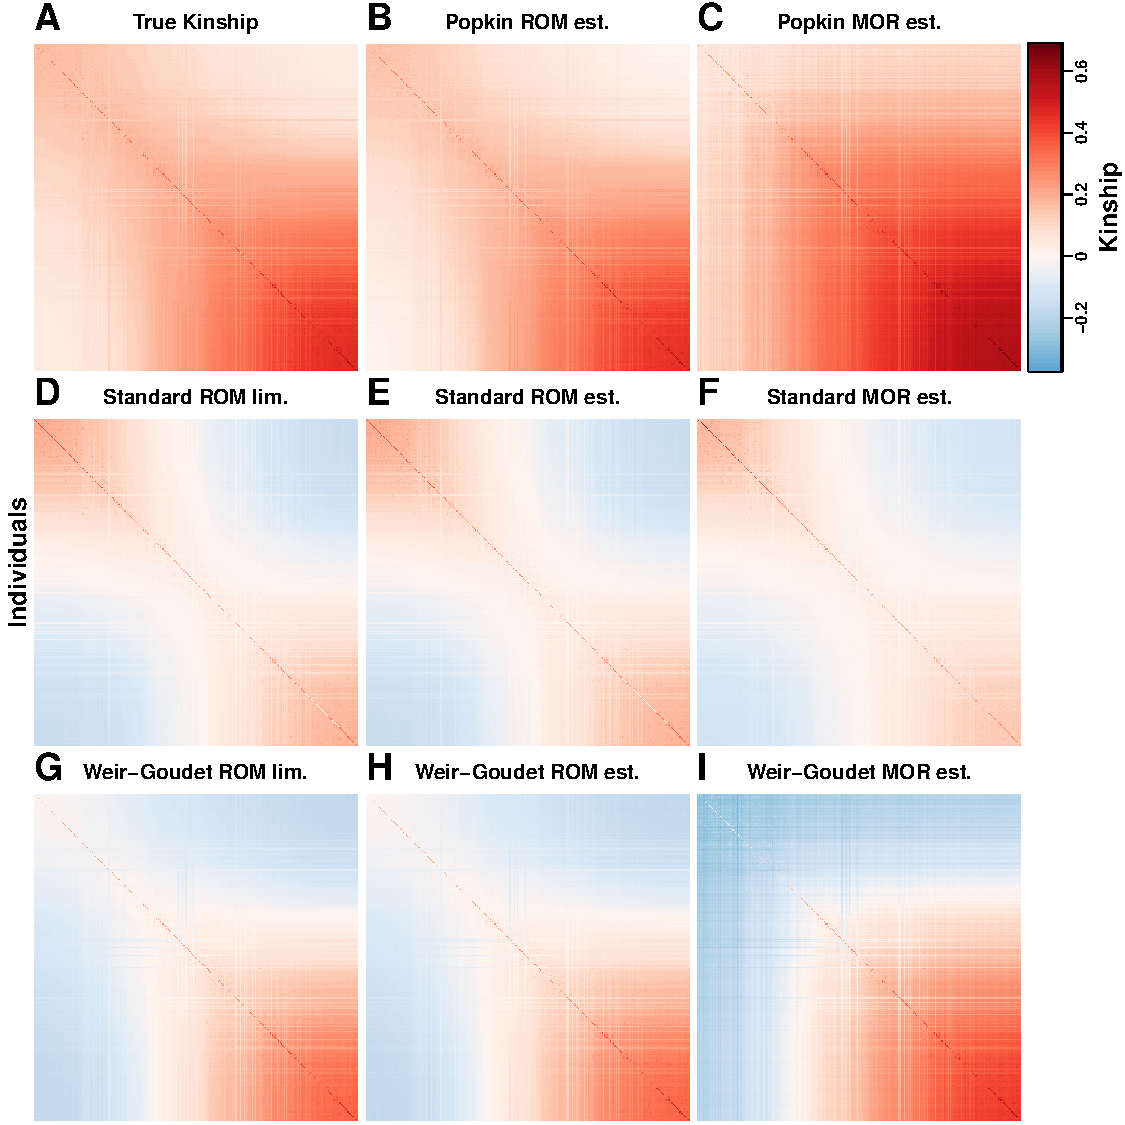
\includegraphics[height=0.8\textheight]{sim-admix-n1000-m100000-k3-f0.3-s0.5-mc100-h0.8-g20-fes/kinship.pdf}
  \caption{
    {\bf Kinship estimates and their limits on the admixed family simulation.}
    Each panel represents a kinship matrix as a heatmap, with each of the $n=1000$ individuals along both x and y axes, and the kinship value presented as color: positive estimates are in red, negative estimates in blue.
    The estimators considered are Popkin, Standard, and Weir-Goudet.
    Each estimator has its limit in the first column (the limit of Popkin is Truth).
    Standard has two variants: ROM (ratio of means) and MOR (mean of ratios).
    Standard MOR does not have a closed-form limit, but in practice matches that of Standard ROM.
  }
  \label{fig:kinship_sim}
\end{figure}

The kinship estimates on this simulation, and the theoretical limits of these estimators, are shown in \cref{fig:kinship_sim}.
The true kinship matrix (\cref{fig:kinship_sim}A) shows the family relatedness as high values concentrated near the diagonal and the ancestry-driven population structure as the broad patterns off-diagonal.
This simulation illustrates the severity of the biases of these estimators, which were previously characterized theoretically \citep{ochoa_estimating_2021}.
Only the Popkin estimator is unbiased (\cref{fig:kinship_sim}B), the rest presenting large negative biases which in turn result in abundant negative estimates.
The Standard kinship estimator (the mean-of-ratios, or MOR, version; \cref{fig:kinship_sim}E), which is the most common estimator in these applications, and the closely related ratio-of-means (ROM) estimator (\cref{fig:kinship_sim}D), both have severe biases that are not only overall downwardly biased, but these biases also vary for every pair of individuals.
The limit of the Standard ROM estimator (\cref{fig:kinship_sim}C), calculated from the true kinship matrix and its known functional form (see Methods), closely matches the previously mentioned estimates obtained from genotypes.
Lastly, the Weir-Goudet estimator has a uniform downward bias (\cref{fig:kinship_sim}H-I).


\begin{figure}[bp!]
  \centering
  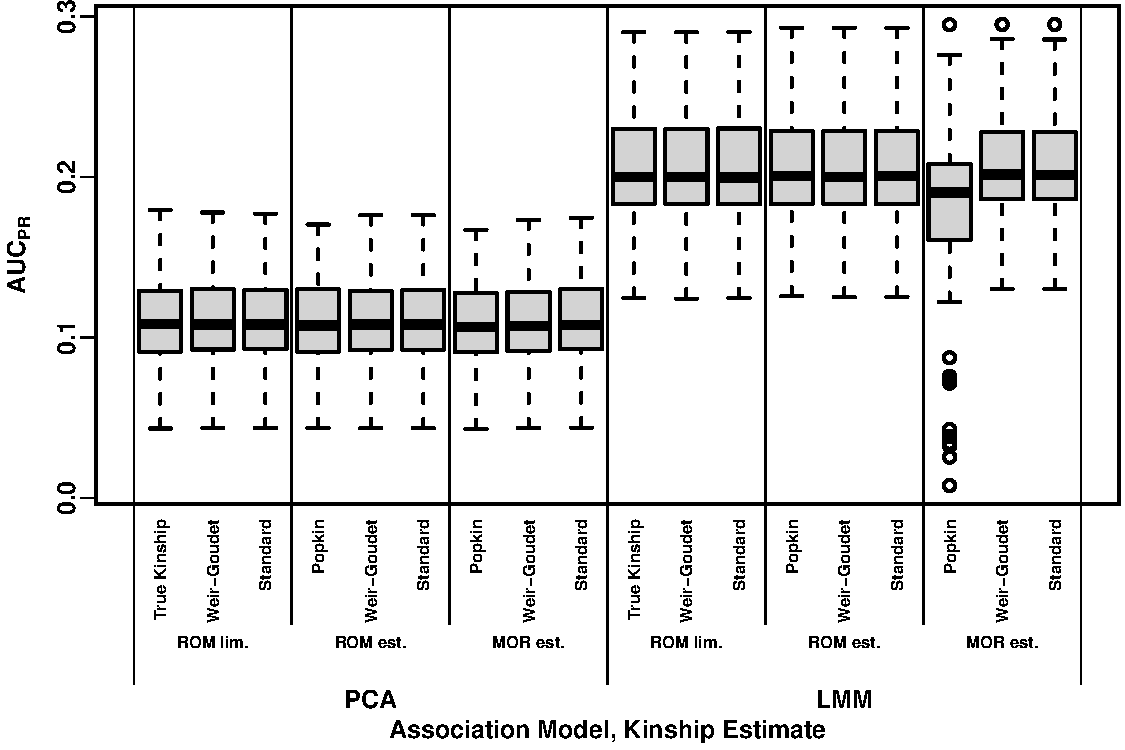
\includegraphics[width=\textwidth]{sim-admix-n1000-m100000-k3-f0.3-s0.5-mc100-h0.8-g20-fes/auc.pdf}
  \caption{
    {\bf Area Under the Precision-Recall Curves ($\auc$) for every combination of association model and kinship estimate on the admixed family simulation.}
    Results based on a single replicate of the random genotype matrix and trait vector.
    Approaches appear to cluster primarily by association model (LMM vs PCA) and whether a kinship estimate was used or not, and do not depend much at all on the form of the bias.
  }
  \label{fig:auc_sim}
\end{figure}

We then performed both LMM and PCA association tests in order to determine if the kinship biases carry over to association biases.
Surprisingly, we found that none of these kinship biases have discernible effects on association performance, as summarized by the Area Under the Precision-Recall Curve ($\auc$; \cref{fig:auc_sim}) and $\rmsd$ (\cref{fig:rmsd_sim}).
The largest difference in performance is explained by the association model used (LMM vs PCA), as expected due to our use of a family simulation, where PCA is expected to perform less well than LMM.
For PCA only, there are no clear differences between the performance of any of the kinship matrices.
In contrast, the LMM results are relatively more sensitive to the use of noisy kinship estimates versus the (noiseless) limits of these estimates, a difference certainly increased by our deliberate use of a small number of simulated loci.
For $\auc$, among the kinship estimator limits, use of the true kinship matrix, the limit of the Weir-Goudet estimator, or the limit of the Standard ROM estimator all result in practically the same performance.
Similarly, among the estimates, the popkin, Weir-Goudet, and Standard ROM estimates result in the same performance, whereas the Standard MOR estimates have a slightly different performance.
For $\rmsd$, all estimates perform similarly except the popkin ROM estimates perform slightly different with a larger variance.


\begin{figure}[bp!]
  \centering
  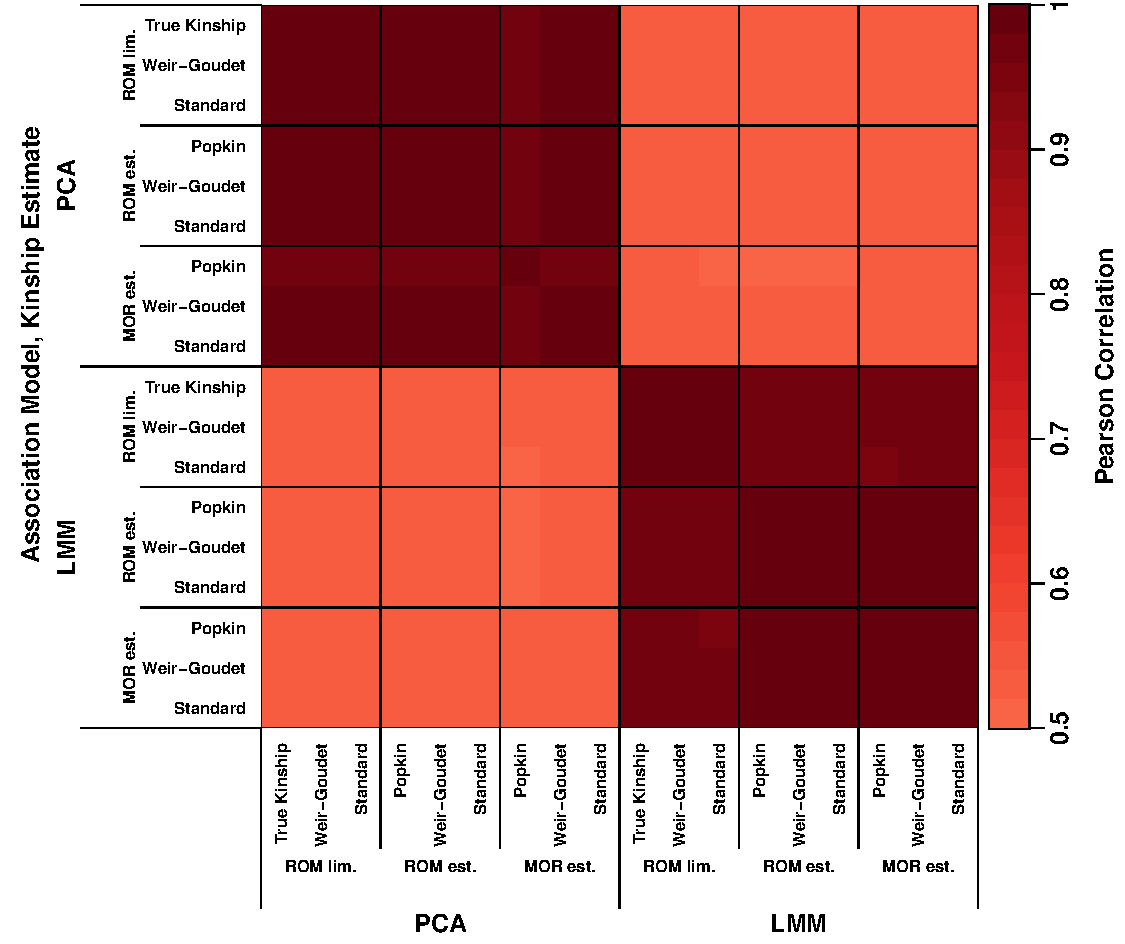
\includegraphics[width=\textwidth]{sim-admix-n1000-m100000-k3-f0.3-s0.5-mc100-h0.8-g20-fes/pvals_cor.pdf}
  \caption{
    {\bf Correlation between p-values of different association models and kinship estimates on the admixed family simulation.}
    The association p-value vector (one value per tested locus) produced by each combination of association model (LMM vs PCA) and kinship matrix (x and y axes) was used to compute Pearson correlations (color).
    Within same type of association model (LMM or PCA), methods are strongly correlated with correlation close to 1 regardless of kinship matrix used.
    }
  \label{fig:pvals_cor_sim}
\end{figure}

To better understand the degree of agreement between the association results of the various kinship matrices, we next measured the agreement between methods at the level of the individual association p-values, summarized using pearson correlation coefficients ($\rho$; \cref{fig:pvals_cor_sim}).
We found that all the kinship matrices yield highly correlated p-values when applied to the same association model (LMM vs PCA), and otherwise mirroring our previous observations based on $\auc$.
The minimum correlation among PCA methods was $0.86$, and among LMMs it was $0.84$.
Within PCA, the cluster that excludes the true kinship matrix and the popkin estimate has nearly identical p-values ($\rho > 0.99$), and inclusion of popkin lowers the minimum correlation to $\rho > 0.93$.
Among LMMs, the cluster that includes the true kinship and the Weir-Goudet and Standard ROM limits also results in practically identical p-values ($\rho \approx 1$).
The LMM cluster that includes the Popkin, Weir-Goudet, and Standard ROM estimators also has $\rho \approx 1$, and separately the cluster with the Standard MOR estimators has $\rho \approx 1$, while the LMM cluster that includes all estimates has $\rho > 0.96$.
Thus, several sets of kinship matrices with different biases result in identical association statistics, within both LMMs and PCA models, while differences are largely driven by the association model used and whether the kinship matrices were estimates or not.

\subsection{Results using 1000 Genomes Project real genotypes}

Now we replicate our previous findings using the real genotypes of 1000 Genomes.
Kinship estimates are shown in \cref{fig:kinship_real}.
Popkin ROM estimates display an approximate nested block structure that arises from the tree relationships between subpopulations (\cref{fig:kinship_real}A; trees were explicitly fit to this data in previous work \citep{yao_limitations_2022}).
However, popkin MOR estimates attain higher values and do not follow the nested blocks tree structure, since kinship between African and non-African populations is higher than kinship within African populations (\cref{fig:kinship_real}B).
Standard estimates have values are closer to zero, and a different bias for each pair of individuals, resulting in higher relative kinship for African compared to non-African populations (\cref{fig:kinship_real}C-D).
Lastly, Weir-Goudet estimates are uniformly smaller than popkin's and attain large negative values (\cref{fig:kinship_real}E-F).

\begin{figure}[bp!]
  \centering
  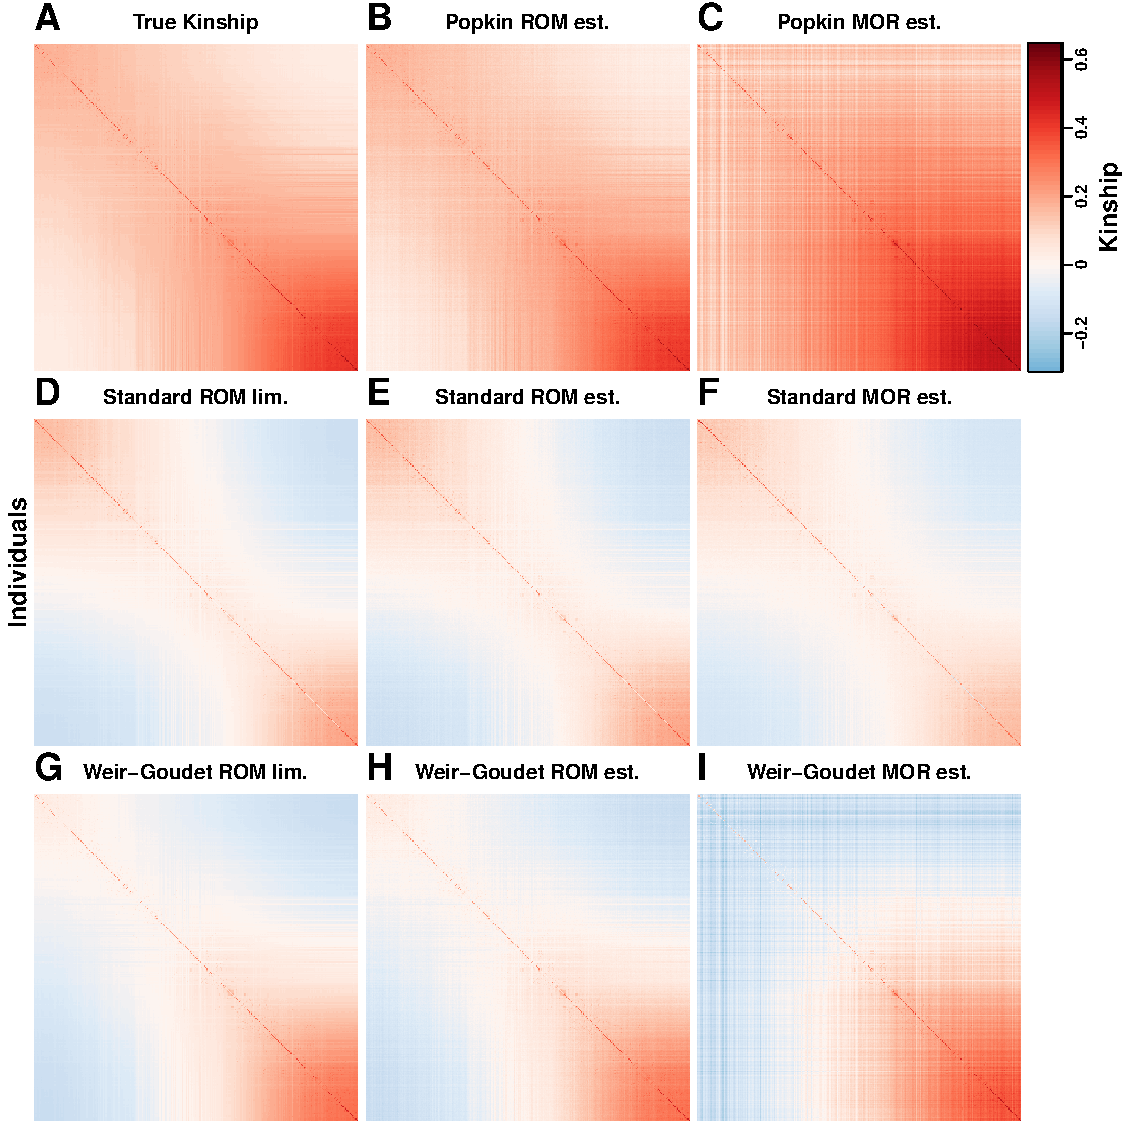
\includegraphics[height=0.8\textheight]{tgp-nygc-autosomes_ld_prune_1000kb_0.3_maf-0.01/kinship.pdf}
  \caption{
    {\bf Kinship estimates and their limits on 1000 Genomes.}
    Each panel represents a kinship matrix as a heatmap, with each individual along both x and y axes, and the kinship value presented as color: positive estimates are in red, negative estimates in blue.
    Superpopulation codes: AFR = African, EUR = European, SAS = South Asian, EAS = East Asian, AMR = Admixed Americans (Hispanics).
    Each estimator (Popkin, Standard, and Weir-Goudet) has two variants: ROM (ratio of means) and MOR (mean of ratios).
    In this visualization the upper range of all panels was capped to the 99 percentile of the diagonal (population inbreeding values) of the popkin MOR estimates.
  }
  \label{fig:kinship_real}
\end{figure}


When we perform PCA and LMM association tests using simulated traits and these kinship estimates, the results are similar to our simulation study: there are no differences between kinship estimators with different biases but of the same type (MOR or ROM) and association model (\cref{fig:auc_real}, \cref{fig:rmsd_real}), with the sole exception of popkin ROM.
However, unlike the admixed family simulation results, here the MOR estimates greatly outperform ROM estimates (both using LMM) for both $\auc$ and $\rmsd$.
We also measured correlations of one between p-values from the same association model and estimator type (MOR or ROM), regardless of bias type (\cref{fig:pvals_cor_real}).

\begin{figure}[bp!]
  \centering
  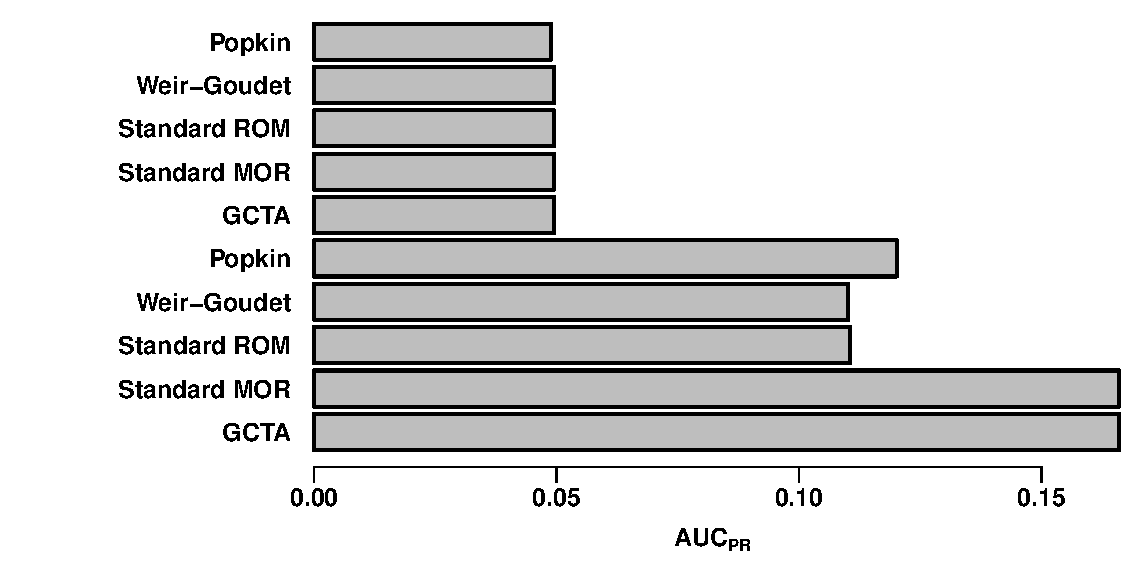
\includegraphics[width=\textwidth]{tgp-nygc-autosomes_ld_prune_1000kb_0.3_maf-0.01/auc.pdf}
  \caption{
    {\bf Area Under the Precision-Recall Curves ($\auc$) for every combination of association model and kinship estimate on 1000 Genomes.}
    Results based on 10 simulated trait replicates (real genotype matrix is fixed).
    Approaches cluster primarily by association model (LMM vs PCA) and whether a kinship estimate was used or not, and do not depend much at all on the form of the bias.
  }
  \label{fig:auc_real}
\end{figure}




\subsection{Theoretical justification of empirical observations under standard kinship bias}

Our empirical observations suggested that the biases of the Standard kinship estimator do not alter association statistics whatsoever; here we provide proof that this is indeed the case.
To eliminate random estimation noise from the analysis (which our empirical evaluations suggest play a minor role), we shall focus exclusively on the limiting bias of the Standard (ROM) kinship estimator.
Our constructive proof identifies the exact conditions that allows the kinship bias to be compensated for, namely that population structure is modeled as a (fixed or random effect) covariate and an intercept term is fit jointly.
More specifically, we find that the coefficients of the intercept and the random effect or PCs (for LMM and PCA, respectively) adapt to the bias, and no other coefficients change.
This is fortunate, as the intercept and random effects or PCs coefficients are nuisance parameters that are most often unreported, while the focal genetic association coefficient and its p-value are completely unchanged by this precise bias.

Our theoretical results only consider the true kinship matrix \kinMat and the limit of the standard kinship estimator (see \textbf{Methods}, \cref{eq:kinship_std_lim}), which can be stated in matrix notation as
$$
\kinMatStdLim
=
\frac{1}{1 - \bar{\varphi}}
\left(
  \kinMat
  + \bar{\varphi} \mathbf{J}
  - \boldsymbol{\varphi} \mathbf{1}^\intercal 
  - \mathbf{1} \boldsymbol{\varphi}^\intercal 
\right)
,
$$
where
$\mathbf{1}$ is a length-$n$ column vector of ones,
$\mathbf{J} = \mathbf{1} \mathbf{1}^\intercal$ is the $n \times n$ matrix full of ones,
$\boldsymbol{\varphi} = \frac{1}{n} \kinMat \mathbf{1}$ is a length-$n$ vector of per-row mean kinship values, and
$\bar{\varphi} = \frac{1}{n^2} \mathbf{1}^\intercal \kinMat \mathbf{1}$ is the overall mean kinship (scalar).
The two kinship matrices are related more succinctly using the $n \times n$ centering matrix,
$$
\mathbf{C}
=
\mathbf{I} - \frac{1}{n} \mathbf{J},
$$
where $\mathbf{I}$ is the $n \times n$ identity matrix.
The limit of the standard kinship estimator is given in terms of a transformation of the true kinship matrix by
\begin{equation}
  \label{eq:kin-std-lim-C}
  \kinMatStdLim
  =
  \frac{1}{1 - \bar{\varphi}}
  \mathbf{C} \kinMat \mathbf{C}
  .
\end{equation}

The centering matrix has been well studied, and we review its properties here.
For any length-$n$ vector $\mathbf{v}$ we have
\begin{align*}
  \mathbf{C} \mathbf{v}
  % =
  % \left(\mathbf{I} - \frac{1}{n} \mathbf{1} \mathbf{1}^\intercal\right) \mathbf{v}
  % =
  % \mathbf{I} \mathbf{v} - \frac{1}{n} \mathbf{1} \mathbf{1}^\intercal \mathbf{v}
  =
  \mathbf{v} - \mathbf{1} \bar{v}
  ,
\end{align*}
where $\bar{v} = \frac{1}{n} \mathbf{1}^\intercal \mathbf{v}$ is the mean value of the elements of $\mathbf{v}$.
Therefore, $\mathbf{v} = \mathbf{1}$ gets transformed to the zero vector, so it is an eigenvector with an eigenvalue of zero:
\begin{align*}
  \mathbf{C} \mathbf{1}
  % =
  % \mathbf{1} - \mathbf{1}
  =
  \mathbf{0}
  .
\end{align*}
Moreover, any vector $\mathbf{v}$ orthogonal to $\mathbf{1}$ has a zero mean element ($\bar{v} = 0$) by hypothesis and it is not altered by $\mathbf{C}$ ($\mathbf{C} \mathbf{v} = \mathbf{v}$).
Therefore, the nullspace of $\mathbf{C}$ is spanned by $\mathbf{1}$.

This centering matrix provides the key insight as to why LMM and PCA approaches are robust to this specific kinship bias, namely that the bias in the random effects (for LMM) or eigenvectors (for PCA) of \kinMatStdLim results in removing the mean values of these covariates only, so fitting the intercept term $\mathbf{1} \alpha$ compensates exactly for this bias.
In the remaining sections we detail this argument, where we construct equivalent solutions under the true and biased kinship matrices.

% First we show the following lemma.

% \begin{lem}
%   $\mathbf{1}$ is in the nullspace of \kinMatStdLim but not of \kinMat.
% \end{lem}

% \begin{proof}
% The vector $\mathbf{1}$ is not in the nullspace of any true kinship matrix \kinMat, since $\kinMat \mathbf{1} \neq \mathbf{0}$, which follows since all kinship values are non-negative and the diagonal of the kinship matrix is strictly positive (it has a minimum value of $\frac{1}{2}$).
% However, $\mathbf{1}$ is in the nullspace of \kinMatStdLim since $\mathbf{C} \mathbf{1} = \mathbf{0}$:
% $$
% \kinMatStdLim \mathbf{1}
% =
% \frac{1}{1 - \bar{\varphi}}
% \mathbf{C} \kinMat \mathbf{C} \mathbf{1}
% =
% \mathbf{0}
% .
% $$
% \end{proof}

% Now we may prove the desired theorem.

% \begin{thm}
%   The rowspace of \kinMat and $\mathbf{1}$ equals rowspace of \kinMatStdLim and $\mathbf{1}$.
% \end{thm}

% \begin{proof}
%   Since $\mathbf{1}$ is in both rowspaces, it suffices to consider vectors $\mathbf{v}$ orthogonal to $\mathbf{1}$, which satisfy $\mathbf{C} \mathbf{v} = \mathbf{v}$.
%   We shall prove below that any such vector is in the nullspace of \kinMat if and only if it is in the nullspace of \kinMatStdLim.
%   Then, since the nullspace of \kinMat and $\mathbf{1}$ is the same as the nullspace of \kinMatStdLim and $\mathbf{1}$, it follows from the fundamental theorem of linear algebra that their rowspaces are also the same.
  
%   If $\mathbf{v}$ is in the nullspace of \kinMat, then $\kinMat \mathbf{v} = \mathbf{0}$.
%   It follows that
%   $$
%   \kinMatStdLim \mathbf{v}
%   =
%   \frac{1}{1 - \bar{\varphi}}
%   \mathbf{C} \kinMat \mathbf{C} \mathbf{v}
%   =
%   \frac{1}{1 - \bar{\varphi}}
%   \mathbf{C} \kinMat \mathbf{v}
%   =
%   \mathbf{0}
%   ,
%   $$
%   so $\mathbf{v}$ is also in the nullspace of \kinMatStdLim.
  
%   Conversely, if $\mathbf{v}$ is in the nullspace of \kinMatStdLim, then $\kinMatStdLim \mathbf{v} = \mathbf{0}$, which implies that
%   $
%   \mathbf{C} \kinMat \mathbf{C} \mathbf{v}
%   =
%   \mathbf{C} \kinMat \mathbf{v}
%   =
%   \mathbf{0}
%   $.
%   Left multiplying by $\mathbf{v}^\intercal$ results in
%   $
%   \mathbf{v}^\intercal \mathbf{C} \kinMat \mathbf{v}
%   =
%   \mathbf{v}^\intercal \kinMat \mathbf{v}
%   =
%   0
%   $, which implies that $\mathbf{v}$ is also in the nullspace of the positive-semidefinite matrix \kinMat, as desired.
%   If \kinMat were positive definite, then no such $\mathbf{v} \ne \mathbf{0}$ would exist (\kinMat would have the trivial nullspace $\{ \mathbf{0} \}$).
% \end{proof}

\subsubsection{Kinship matrix square root}

% https://en.wikipedia.org/wiki/Square_root_of_a_matrix

Here we shall consider decompositions of positive semidefinite matrices of the form $\mathbf{\Sigma} = \mathbf{B} \mathbf{B}^\intercal$, which are guaranteed to exist.
We denote such a $\mathbf{B}$ as a square root of $\mathbf{\Sigma}$, or in short $\mathbf{B} = \mathbf{\Sigma}^\frac{1}{2}$.
These square roots of $\mathbf{\Sigma}$ are not unique, which is not a problem for our following argument; any such square root will work.
(Note that there are alternate definitions of matrix square roots, such as $\mathbf{\Sigma} = \mathbf{B} \mathbf{B}$, but due to its connection to covariance, the definition $\mathbf{\Sigma} = \mathbf{B} \mathbf{B}^\intercal$ we adopted is most natural for this work and the notation $\mathbf{B} = \mathbf{\Sigma}^\frac{1}{2}$ simplifies our arguments.)

Given a square root of the true kinship matrix, $\kinMat^\frac{1}{2}$, we can construct a square root of the limit of the standard kinship estimator as
\begin{equation}
  \label{eq:eq:kin-std-lim-C-sqrt}
  \left( \kinMatStdLim \right)^\frac{1}{2}
  =
  \frac{1}{ \sqrt{ 1 - \bar{\varphi} } }
  \mathbf{C} \kinMat^\frac{1}{2}
  .
\end{equation}
This matrix square root can be verified to satisfy
$\left( \kinMatStdLim \right)^\frac{1}{2} \left( \left( \kinMatStdLim \right)^\frac{1}{2} \right)^\intercal = \kinMatStdLim$
as given in \cref{eq:kin-std-lim-C}.

\subsubsection{The LMM genetic association model}

In genetic association we are given data for $n$ individuals, namely a length-$n$ vector of trait values $\mathbf{y}$, which correspond to a quantitative trait, and a length-$n$ vector $\mathbf{x}_i$ of genotypes at each locus $i$.
These genotypes are encoded as dosages for a given risk allele that varies for each locus $i$, so it takes on the values of 0, 1, or 2 for diploid individuals.
The goal is to determine if there is a significant association between the trait and the genotype vectors.
Most genetic association models are formulated as, or are equivalent to, regression models.

The LMM regression model is given by
\begin{equation}
  \label{eq:lmm_gwas}
  \mathbf{y}
  =
  \alpha \mathbf{1} + \beta \mathbf{x}_i + \mathbf{s} + \boldsymbol{\epsilon}
  ,
\end{equation}
where $\alpha$ is the intercept coefficient,
$\beta$ is the genetic effect coefficient,
$\boldsymbol{\epsilon}$ are random independent residuals ($\boldsymbol{\epsilon} \sim \text{Normal}(\mathbf{0}, \sigma^2_\epsilon \mathbf{I})$ for some $\sigma^2_\epsilon$ fit to the data),
and the random effect satisfies \citep{sul_population_2018}
$$
\mathbf{s} \sim \text{Normal} \left( \mathbf{0}, \sigma^2 \kinMat \right),
$$
where $\sigma^2$ is also fit to the data.
The dependence of the model on \kinMat is clearer by writing it equivalently as
\begin{equation}
  \label{eq:lmm_gwas2}
  \mathbf{y}
  =
  \alpha \mathbf{1} + \beta \mathbf{x}_i + \sigma \kinMat^\frac{1}{2} \mathbf{r} + \boldsymbol{\epsilon}
  ,
\end{equation}
where $\mathbf{r} \sim \text{Normal} \left( \mathbf{0}, \mathbf{I} \right)$.
The equivalence of \cref{eq:lmm_gwas} and \cref{eq:lmm_gwas2} follows since $\mathbf{r}$ being Multivariate Normal implies that the affine transformation $\mathbf{s} = \sigma \kinMat^\frac{1}{2} \mathbf{r}$ is also Multivariate Normal, with matching mean and covariance of the desired $\mathbf{s}$, namely
\begin{align*}
  \E[ \mathbf{s} ]
  &=
    \sigma \kinMat^\frac{1}{2} \E[ \mathbf{r} ]
    = \mathbf{0},
  \\
  \Cov( \mathbf{s} )
  &= \left( \sigma \kinMat^\frac{1}{2} \right) \Cov( \mathbf{r} ) \left( \sigma \kinMat^\frac{1}{2} \right)^\intercal
    = \sigma^2 \kinMat
    .
\end{align*}
Note that the equivalence holds for every square root of \kinMat (all $\mathbf{s} = \sigma \kinMat^\frac{1}{2} \mathbf{r}$ are equal in distribution), since the only requirement for equivalence,
$\left( \kinMat^\frac{1}{2} \right) \left( \kinMat^\frac{1}{2} \right)^\intercal = \kinMat$,
is satisfied by hypothesis.

\subsubsection{Equivalent LMM fit under standard kinship bias}

In the LMM of \cref{eq:lmm_gwas2}, $\mathbf{y}$, $\mathbf{x}_i$, and \kinMat are given, while the coefficients $\alpha$, $\beta$, $\sigma$, and the random effects $\mathbf{r}$ and $\boldsymbol{\epsilon}$ are fit to this data.
This data is typically fit using maximum likelihood (ML) or restricted maximum likelihood (REML) \citep{kang_efficient_2008}; our argument covers any likelihood-based approach, since we will establish a parameter map between both models that results in equal likelihoods for every parameter set in the map.

We shall consider two model fits, one where \kinMat is given, while in the other we provide $\kinMat' = \kinMatStdLim$ instead.
The first fit will result in the unprimed variables below, while we distinguish the second fit using primed variables, namely:
\begin{align*}
  \mathbf{y}
  &=
    \alpha \mathbf{1} + \beta \mathbf{x}_i + \sigma \kinMat^\frac{1}{2} \mathbf{r} + \boldsymbol{\epsilon}
  \\
  &=
    \alpha' \mathbf{1} + \beta' \mathbf{x}_i + \sigma' \left( \kinMat' \right)^\frac{1}{2} \mathbf{r}' + \boldsymbol{\epsilon}'
    .
\end{align*}
Now we shall construct coefficients for the second model that result in the same fit to the data, including the same likelihood, as the first model.
We achieve this by first setting
$\beta' = \beta$,
$\boldsymbol{\epsilon}' = \boldsymbol{\epsilon}$,
and
$\mathbf{r}' = \mathbf{r}$.
Note that the previous equal random effects (including residuals) immediately results in the same likelihood for both models.
The only parameters left to construct are $\alpha'$ and $\sigma'$, which must satisfy
$$
\alpha \mathbf{1}  + \sigma \kinMat^\frac{1}{2} \mathbf{r}
=
\alpha' \mathbf{1} + \sigma' \left( \kinMat' \right)^\frac{1}{2} \mathbf{r}
.
$$
Next we substitute $\kinMat' = \kinMatStdLim$ using the matrix square root determined in terms of \kinMat in \cref{eq:eq:kin-std-lim-C-sqrt}, which results in
$$
\alpha \mathbf{1} + \sigma \kinMat^\frac{1}{2} \mathbf{r}
=
\alpha' \mathbf{1} + \sigma'
\frac{1}{ \sqrt{ 1 - \bar{\varphi} } }
\mathbf{C} \kinMat^\frac{1}{2}
\mathbf{r}
.
$$
The unknowns are solved for by left-multiplying, in turns, by $\mathbf{C}$ (which makes terms with $\mathbf{1}$ vanish) and by $\mathbf{1}^\intercal$ (which makes the term with $\mathbf{C}$ vanish).
In the first case, left-multiplying by $\mathbf{C}$ results in
$$
\sigma \mathbf{C} \kinMat^\frac{1}{2} \mathbf{r}
=
\sigma'
\frac{1}{ \sqrt{ 1 - \bar{\varphi} } }
\mathbf{C} \kinMat^\frac{1}{2}
\mathbf{r}
,
$$
so the only value of the scalar $\sigma'$ that satisfies this equation is
$$
\sigma'
=
\sigma \sqrt{ 1 - \bar{\varphi} }
.
$$
In the second case, left-multiplying by $\mathbf{1}^\intercal$, while noting that $\mathbf{1}^\intercal \mathbf{1} = n$, and solving for $\alpha'$ results in
$$
\alpha'
=
\alpha  + \sigma \frac{1}{n} \mathbf{1}^\intercal \kinMat^\frac{1}{2} \mathbf{r}
.
$$
Note that the last equation can also be written as
$$
\alpha'
=
\alpha  + \eta
,
\quad\quad
\eta \sim \text{Normal}( 0, \sigma^2 \bar{\varphi} )
,
$$
since $\eta = \sigma \frac{1}{n} \mathbf{1}^\intercal \kinMat^\frac{1}{2} \mathbf{r}$ is a scalar random Normal variable (because it is a sum of marginals of a Multivariate Normal, each of which are Normal) with mean zero (because $\mathbf{r}$ had mean zero) and the stated variance (since $\Var( \sigma \frac{1}{n} \mathbf{1}^\intercal \kinMat^\frac{1}{2} \mathbf{r} ) = ( \sigma \frac{1}{n} \mathbf{1}^\intercal \kinMat^\frac{1}{2}) \Cov( \mathbf{r} ) ( \sigma \frac{1}{n} \mathbf{1}^\intercal \kinMat^\frac{1}{2} )^\intercal$, $\Cov( \mathbf{r} ) = \mathbf{I}$, and $\frac{1}{n^2} \mathbf{1}^\intercal \kinMat \mathbf{1} = \bar{\varphi}$).


We just determined that every solution in terms of the true kinship matrix (including every combination of fixed coefficients and random effects) has a corresponding solution in terms of the limit of the standard kinship estimator, which has equal likelihood and equal fit to the data.
This includes the optimal solution, whether determined by the ML or REML criteria.
In both cases, the coefficient for the genetic effect is identical ($\beta' = \beta$ above), and because the fit to the data is also equal (in terms of likelihood and/or residuals), the association p-value is also equal (whether determined from the likelihood or from residuals).
Thus, while two coefficients (the intercept $\alpha$ and the random effect variance scale $\sigma^2$) vary depending on whether the true or the limit of the biased standard kinship estimator are used, these are both nuisance parameters as far as the association test is concerned.
The focal genetic effect coefficient and significance statistic are both invariant under this particular kinship bias compared to using the true kinship matrix.

\subsubsection{The PCA genetic association model}

The argument we just presented for LMM equivalence can be made with small changes for the PCA regression model, since these two models are so similar.
Here we shall state the PCA model and elaborate on its strong connection to the LMM model, which has been presented before in similar forms \citep{astle_population_2009, hoffman_correcting_2013}.

The PCA regression model is
\begin{equation}
  \label{eq:pca_gwas}
  \mathbf{y}
  =
  \alpha \mathbf{1} + \beta \mathbf{x}_i + \mathbf{U}_d \boldsymbol{\gamma}_d + \boldsymbol{\epsilon}
  ,
\end{equation}
where
$d$ is the number of principal components,
$\mathbf{U}_d$ is the $n \times d$ matrix of top eigenvectors (often refered to as ``principal components'' in genetics),
and $\boldsymbol{\gamma}_d$ is a length-$d$ vector of coefficients for each eigenvector.
Note that the only difference from the LMM model (\cref{eq:lmm_gwas2}) is the replacement of $\sigma \kinMat^\frac{1}{2} \mathbf{r}$ with $\mathbf{U}_d \boldsymbol{\gamma}_d$ here.

Before proceeding with our proof for invariance under the PCA model, to enhance our intuition of these two models, we present the relationship between eigendecomposition and matrix square roots, which helps us connect the PCA model firmly to the LMM.
Denote the eigendecomposition of the true kinship matrix as
$$
\kinMat = \mathbf{U} \mathbf{\Lambda} \mathbf{U}^\intercal,
$$
where $\mathbf{U}$ is the complete $n \times n$ matrix of eigenvectors, and
$\mathbf{\Lambda}$ is the $n \times n$ diagonal matrix of eigenvalues.
%The matrix of eigenvectors is orthogonal, so $\mathbf{U}^{-1} = \mathbf{U}^\intercal$.
Therefore, one square root of \kinMat is given by
$$
\kinMat^\frac{1}{2}
=
\mathbf{U} \mathbf{\Lambda}^\frac{1}{2}
,
$$
where $\mathbf{\Lambda}^\frac{1}{2}$ contains the square roots of each eigenvalue along the diagonal.
This equation reveals that the LMM model in \cref{eq:lmm_gwas2} can be written in terms of the eigendecomposition, and thus resemble the PCA model even more closely, since
$$
\sigma \kinMat^\frac{1}{2} \mathbf{r}
=
\sigma \mathbf{U} \mathbf{\Lambda}^\frac{1}{2} \mathbf{r}
=
\mathbf{U} \boldsymbol{\gamma}
,
$$
so that the length-$n$ vector $\boldsymbol{\gamma}$ of coefficients for all the $n$ eigenvectors is given by
$
\boldsymbol{\gamma} = \sigma \mathbf{\Lambda}^\frac{1}{2} \mathbf{r}
$.
Thus, the PCA model attempts to fit coefficients only for the top $d$ eigenvectors, whereas the LMM model effectively fits all of these coefficients by constraining them to a distribution.

\subsubsection{Approximately equivalent PCA fit under standard kinship bias}

We shall again consider two alternate model fits, here based on the PCA model of \cref{eq:pca_gwas}, one where the eigenvector matrix $\mathbf{U}_d$ corresponds to the true kinship matrix, and in the other $\mathbf{U}_d'$ corresponds to the biased limit of the standard kinship estimator.
They key approximation is that
$$
\mathbf{U}_d' \approx \mathbf{C} \mathbf{U}_d,
$$
which is not strictly equal (since $\mathbf{C} \mathbf{U}$ is not orthogonal, as eigenvectors must be), but we have found it to be a good approximation in practice.

The two model fits we are considering are
\begin{align*}
  \mathbf{y}
  &=
    \alpha \mathbf{1} + \beta \mathbf{x}_i + \mathbf{U}_d \boldsymbol{\gamma}_d + \boldsymbol{\epsilon}
  \\
  &=
    \alpha' \mathbf{1} + \beta' \mathbf{x}_i + \mathbf{U}_d' \boldsymbol{\gamma}_d' + \boldsymbol{\epsilon}'
    ,
\end{align*}
and we again assume that the focal parameter $\beta' = \beta$ and the residuals $\boldsymbol{\epsilon}' = \boldsymbol{\epsilon}$ are equal.
Eliminating the resulting shared terms, and replacing $\mathbf{U}_d' = \mathbf{C} \mathbf{U}_d$ (assuming that our approximation holds exactly) results in the remaining coefficients having to satisfy
$$
\alpha \mathbf{1} + \mathbf{U}_d \boldsymbol{\gamma}_d
=
\alpha' \mathbf{1} + \mathbf{C} \mathbf{U}_d \boldsymbol{\gamma}_d'.
$$
We solve for the missing coefficients by left-multiplying by $\mathbf{C}$ and $\mathbf{1}^\intercal$ as before, which here ultimately results in
\begin{align*}
  \boldsymbol{\gamma}_d'
  =
    \boldsymbol{\gamma}_d
  ,
  \quad\quad
  \alpha'
  =
    \alpha + \frac{1}{n} \mathbf{1}^\intercal \mathbf{U}_d \boldsymbol{\gamma}_d
    .
\end{align*}
Thus, as for LMM, here the nuisance intercept coefficient compensates for the bias in the eigenvectors.

The PCA regression is an ordinary multiple linear regression, which is fit by minimizing the sum of square residuals.
Since the residuals were equal in both models, then the optimal solution in one model maps to the optimal solution in the other model as well.
The p-value of the genetic effect is usually calculated using a chi-squared test or an F-test, both of which depend only on the residuals and the degrees of freedom, all of which are invariant under the solution parameter map we constructed.
Therefore, both the focal genetic effect coefficient $\beta$ and its p-value are invariant under this particular kinship bias compared to using the true kinship matrix.
However, the result for PCA relies on an approximation, whereas for LMM it was exact.

\subsection{Proof that association based on Weir-Goudet and true kinship are equivalent}

The limiting bias of the Weir-Goudet (WG) estimator (see Methods, \cref{eq:wg_lim}) is given in terms of the true kinship matrix by
\begin{equation}
  \label{eq:wg_lim_mat}
  \kinMatWGLim
  =
  \frac{1}{1-\tilde{\varphi}}( \kinMat - \tilde{\varphi}\mathbf{J})
  .
\end{equation}
Our strategy for proving the association equivalence under both kinship matrices is to construct a random effect structured as the true kinship matrix from a random effect structured as WG.
Although we were unable to calculate a matrix square root for the WG limit in terms of the true kinship matrix, we found that this alternate derivation for LMMs proves the desired result and leads to strikingly analogous equations for the variance scale $\sigma^2$ and intercept $\alpha$ between both models, where the only difference ultimately is the replacement of the mean kinship $\bar{\varphi}$ in the standard estimator results with $\tilde{\varphi}$ for WG.
We were unable to prove the PCA case with this strategy.

\subsubsection{Constructing random effects with true kinship structure from Weir-Goudet structure}

Solving for the true kinship matrix in \cref{eq:wg_lim_mat}, we obtain
\begin{equation}
  \label{eq:kin_mat_true_wg}
  \kinMat = (1-\tilde{\varphi}) \kinMatWGLim + \tilde{\varphi} \mathbf{J}.
\end{equation}
Let the random effect from the LMM using the WG limit be
$$
\mathbf{s}^\text{WG} \sim \text{Normal} \left( \mathbf{0}, \sigma^2_\text{WG} \kinMatWGLim \right),
$$
where $\sigma^2_\text{WG}$ is a parameter fit to the data.
The Normal distribution above requires that \kinMatWGLim be positive definite, a fact that is proven for arbitrary true kinship matrices (except for one degenerate case) in \cref{sec:wg_posdef}.
We desire to construct a random effect such that 
$
\mathbf{s} \sim \text{Normal} \left( \mathbf{0}, \sigma^2 \kinMat \right),
$
where again $\sigma^2$ has been fit to the data.
\cref{eq:kin_mat_true_wg} suggest a relationship of the form
$$
\mathbf{s} = \mathbf{s}^\text{WG} + \eta \mathbf{1},
$$
where $\eta$ is a random scalar drawn independently from a Normal distribution,
$$
\eta \sim \text{Normal}( 0,\sigma_{\eta}^2),
$$
where $\sigma_{\eta}^2$ is yet to be determined.
This constructed $\mathbf{s}$ is indeed Multivariate Normal since $\eta \mathbf{1}$ is a (degenerate) Multivariate Normal and the sum of two Multivariate Normal variables is itself a Multivariate Normal variable.
All that is left is to match the mean of covariance of the desired $\mathbf{s}$, namely
\begin{align*}
  \E[ \mathbf{s} ]
  &=
    \E \left[ \mathbf{s}^\text{WG} \right] + \E [ \eta ] \mathbf{1}
    =
    \mathbf{0},
  \\
  \Cov( \mathbf{s} )
  &=
    \Cov \left( \mathbf{s}^\text{WG} \right) + \Var ( \eta ) \mathbf{J}
    \\
  &= 
    \sigma^2_\text{WG} \kinMatWGLim + \sigma_{\eta}^2 \mathbf{J}
    =
    \sigma^2 \kinMat
    ,
\end{align*}
which is achieved with $\sigma^2 = \sigma^2_\text{WG} / ( 1 - \tilde{\varphi} )$ and $\sigma_{\eta}^2 = \tilde{\varphi} \sigma^2$.

\subsubsection{Equivalent LMM fit under Weir-Goudet kinship bias}

Similarly to the case for the standard kinship estimator, we consider two equivalent LMM fits, one with $\mathbf{s}$ from the true kinship matrix, the other with $\mathbf{s}' = \mathbf{s}^\text{WG}$ from the WG limit:
$$
\mathbf{y}
=
\alpha \mathbf{1} + \beta \mathbf{x}_i + \mathbf{s} + \boldsymbol{\epsilon}
=
\alpha' \mathbf{1} + \beta' \mathbf{x}_i + \mathbf{s}' + \boldsymbol{\epsilon}'
.
$$
As before, our empirical results motivate that $\beta = \beta', \boldsymbol{\epsilon} = \boldsymbol{\epsilon}'$, and only $\alpha'$ is left, which must satisfy
$$
\alpha \mathbf{1} + \mathbf{s}
=
\alpha' \mathbf{1} + \mathbf{s}'
.
$$
We now substitute our constructed $\mathbf{s} = \mathbf{s}' + \eta \mathbf{1}$, where $\eta$ is as determined in the previous subsection, which after simplifying yields
$$
\alpha \mathbf{1} + \eta \mathbf{1}
=
\alpha' \mathbf{1}
.
$$
Note $\mathbf{s}'$ drops out of the equation, which follows from having previously selected its variance appropriately to match that of the model for the true kinship matrix, namely
$$
\sigma' = \sigma \sqrt{ 1 - \tilde{\varphi} },
$$
where $\sigma' = \sigma_\text{WG}$, which agrees with the solution we found earlier for the standard kinship estimator, expect replacing $\bar{\varphi}$ with $\tilde{\varphi}$.
Lastly, the relation between intercepts is
$$
\alpha' = \alpha + \eta,
$$
which again resembles the solution for the standard model, where both draw a random variable with mean zero, except the earlier variance of $\sigma^2 \bar{\varphi}$ is replaced with $\sigma^2 \tilde{\varphi}$ here.
As before, these results imply that the association statistics are invariant to the choice between the true and WG limit kinship matrices.

% \subsubsection{Approximately equivalent PCA fit under Weir-Goudet kinship bias}

% ...
% The rest of the proof for PCA association equivalence under Weir-Goudet kinship bias is similar to the one for standard kinship bias and is omitted.



\section{Discussion}

% association robust to bias type (empirical and theory / summary)
Previous research showed that commonly used kinship estimators are biased, and that these biases can be large (\citet{ochoa_estimating_2021}; \cref{fig:kinship_sim}).
We initiated the present work under the hypothesis that these kinship biases would affect association testing, but surprisingly find that association is unaffected by these kinship biases.
We then prove theoretically that it is the intercept and population structure (random effect or PCs) coefficients that compensate for the bias, and result in identical genetic effect coefficients and significance statistics.

% popkin is less numerically stable
Given that kinship bias type is not important for association studies, we are free to choose a kinship estimator based on other properties.
The biased standard kinship matrix may be more desirable than the popkin estimator based on the numerical stability we observed in our simulations.
In particular, while theory shows that the solutions should be the same for all estimators of the same type, we find that popkin's statistics disagree more often from the standard and WG estimators, namely LMM association with popkin MOR (admixed family simulation, \cref{fig:auc_sim}, \cref{fig:rmsd_sim}) and popkin ROM (1000 Genomes, \cref{fig:rmsd_real}).
The standard kinship matrix is orthogonal to the intercept, because of the centering operation applied to obtain it in our theoretical results, whereas the popkin and true kinship matrix are not orthogonal to the intercept.
Thus, PCA regression with the eigenvectors of the standard kinship matrix is more numerically stable (because more covariates are linearly independent) than the popkin counterpart.
We believe that the observed popkin disagreemnts in LMMs are due to poor convergence of that algorithm in those cases.

% MOR weirdness
We also found that all MOR estimators perform better in the LMM association (and overall) compared to the ROM versions in the 1000 Genomes evaluation.
Perhaps this is expected because out trait simulation follows the ``fixed effect sizes'' model, in which rare variants have larger coefficients, and the MOR estimators also weigh rare variants more highly in estimating kinship coefficients.
This effect was not observed in the admixed family simulation, where MOR and ROM versions gave similar kinship estimates and performed similarly, compared to the real data evaluation, where kinship estimates were also strikingly different.
However, only the popkin ROM estimator is unbiased (\cref{fig:kinship_sim}B), so it is unclear why the biased popkin MOR estimator performs better in this setting.
One potential explanation is that our kinship model assumes that all variants were preexisting in the MRCA population, whereas rare variants in human data are known to be very recent mutations, and thus their effective kinship matrix is different than that of ancestral variants.
Therefore, despite its biases, it is possible that the popkin MOR estimator is more accurately capturing the kinship matrix of these rare variants and thus modeling them better in association tests, particularly in LMMs where the effect is most pronounced.

% conclusion / take away
In this study, we show empirically and theoretically that association tests are invariant to the use of common kinship estimators that are biased as well as a more recent unbiased estimator.
% future work / implication beyond this work
The theoretical underpinnings of our proof show that the same is expected of any generalized linear model with the same setup, namely intercept and population structure with coefficients that are nuisance variables.
However, heritability estimation requires unbiased estimates of the random effect coefficient ($\sigma^2$), so our results prove that it will be biased when the standard kinship estimator is used, as it is using GCTA \citep{yang_gcta:_2011, yang_advantages_2014}.
Nevertheless, heritability estimation is a complex problem and its full study is beyond the scope of this work.
Overall, we have described an unexpected robustness of association studies, and our theoretical understanding of this result may help guide future improvements for association and other related models.



\section*{Declaration of interests}
The authors declare no competing interests.

\section*{Acknowledgments}
This work was funded in part by the Duke University School of Medicine Whitehead Scholars Program, a gift from the Whitehead Charitable Foundation.
The 1000 Genomes data were generated at the New York Genome Center with funds provided by NHGRI Grant 3UM1HG008901-03S1.

\section*{Web resources}
plink2, \url{https://www.cog-genomics.org/plink/2.0/}\\
GCTA, \url{https://yanglab.westlake.edu.cn/software/gcta/}\\
bnpsd, \url{https://cran.r-project.org/package=bnpsd}\\
simfam, \url{https://cran.r-project.org/package=simfam}\\
simtrait, \url{https://cran.r-project.org/package=simtrait}\\
popkin, \url{https://cran.r-project.org/package=popkin}\\
popkinsuppl, \url{https://github.com/OchoaLab/popkinsuppl}

\section*{Data and code availability}
The data and code generated during this study are available on GitHub at \url{https://github.com/OchoaLab/bias-assoc-paper}.
The high-coverage version of the 1000 Genomes Project was downloaded from \url{ftp://ftp.1000genomes.ebi.ac.uk/vol1/ftp/data_collections/1000G_2504_high_coverage/working/20190425_NYGC_GATK/}.


\printbibliography


\begin{appendices}
  \appendix

  \appendixpage
  
  \section{Justification for popkin generalizations.}

  \label{sec:popkin_w_justif}

  The popkin estimator in \cref{eq:popkin} has been generalized in this work to include locus weights $w_i$.
  The original formulation had $w_i=1$ for all loci $i$ \citep{ochoa_estimating_2021}.
  Recalling from that original work that
  $$
  \E[ (\xij-1)(\xij[k]-1) - 1 ] = 4 \pit ( 1 - \pit ) ( \kt - 1 ),
  $$
  then for fixed $w_i$ we get
  \begin{align*}
    \E[ \Ajk ]
    &=
      v_m ( \kt - 1 )
      , \\
    v_m
    &=
      \frac{4}{m} \sum_{i=1}^m w_i \pit ( 1 - \pit )
      .
  \end{align*}
  Therefore, as before all the unknowns \pit and now also the (known) weights $w_i$ collapse into a single parameter $v_m$, which is estimated under the original assumption that the minimum kinship is zero, giving $\AMinHat = -v_m$, so that
  $$
  \ktHatNamed{popkin-ROM}
  =
  1 - \frac{\Ajk}{\AMinHat}
  \toas
  \kt
  $$
  as desired.

  The MOR case of $w_i = (\pith (1-\pith))^{-1}$ does not fit the previous case because this $w_i$ is a random variable (it is a function of the genotypes).
  The term of interest $w_i ( (\xij-1)(\xij[k]-1) - 1 )$ is a ratio of random variables whose expectation does not have a closed form.
  In this case, we rely on the first-order approximation to this expectation, namely
  \begin{align*}
    \E \left[ \frac{ (\xij-1)(\xij[k]-1) - 1 }{ \pith (1-\pith) } \right]
    &\approx
      \frac{ \E[ (\xij-1)(\xij[k]-1) - 1 ] }{ \E[ \pith (1-\pith) ] }
    \\
    &=
      \frac{ 4 \pit ( 1 - \pit ) ( \kt - 1 ) }{ \pit (1-\pit) ( 1 - \bar{\varphi} ) }
    \\
    &=
      \frac{ 4 ( \kt - 1 ) }{ 1 - \bar{\varphi} }
  ,
  \end{align*}
  where the expectation of $\pith (1-\pith)$ was calculated previously \citep{ochoa_estimating_2021}.
  In this case the expectation of \Ajk, summing across loci, is also approximated by
  $$
  \E[ \Ajk ]
  \approx
  \frac{ 4 ( \kt - 1 ) }{ 1 - \bar{\varphi} }
  .
  $$
  The same strategy as before applies to estimate the unknown factor $4 / ( 1- \bar{\varphi} )$, namely that if the minimum kinship is zero then $\AMinHat \approx - 4 / ( 1- \bar{\varphi} )$, resulting in
  $$
  \ktHatNamed{popkin-MOR}
  =
  1 - \frac{\Ajk}{\AMinHat}
  \approx
  \kt
  .
  $$

  \section{Connection between popkin and standard kinship estimator}

  \label{sec:conn_popkin_std}  

  Since the conection we discovered holds when data is complete but not under missingness, to determine necessary conditions, here we introduce more complete forms of the estimators that handle missingness.
  The generalized popkin estimator (including both ROM and MOR special cases) is
  \begin{equation*}
    %\label{eq:popkin_miss}
    \begin{split}
      A_{ijk}
      &=
        I_{ij} I_{ik} ( (\xij-1)(\xij[k]-1) - 1 )
      , \\
      \Ajk
      &=
        \frac{1}{m_{jk}} \sum_{i=1}^m w_i A_{ijk}
        , \\
      m_{jk}
      &=
        \sum_{i=1}^m I_{ij} I_{ik}
        ,
    \end{split}
  \end{equation*}
  where $I_{ij} = 1$ if \xij is not missing, 0 otherwise (this way missing \xij can be treated as having any finite value and not contribute to the estimator).
  Note that only loci where both genotypes ($\xij$ and $\xij[k]$) are non-missing are included in the above average, and $m_{jk}$ counts the total number of such loci.
  The ancestral allele frequency estimator with missingness is
  \begin{align*}
    \pith
    &=
      \frac{1}{2 n_i} \sum_{j=1}^n I_{ij} \xij
      , \\
    n_i
    &=
      \sum_{j=1}^n I_{ij}
      ,
  \end{align*}
  which averages over individuals rather than loci, so its denominator is the number of non-missing individuals at this locus.
  Let us compute some averages of the generalized popkin estimator.
  Since the result we want holds at every locus separately, let us formulate the averages of interest at locus $i$ only:
  \begin{align*}
    \bar{A}_{ij}
    &=
      \frac{1}{n} \sum_{k=1}^n A_{ijk}
      =
      I_{ij} \frac{n_i}{n} ( ( \xij - 1 )( 2 \pith - 1 ) - 1 )
      , \\
    \bar{A}_i
    &=
      \frac{1}{n} \sum_{k=1}^n \bar{A}_{ij}
      =
      - \left( \frac{n_i}{n} \right)^2 4 \pith ( 1 - \pith )
      .
  \end{align*}
  Therefore, the combination of interest is:
  \begin{align*}
    A_{ijk} + \bar{A}_i - \bar{A}_{ij}  - \bar{A}_{ik}
    % &=
    %   I_{ij} I_{ik} ( (\xij-1)(\xij[k]-1) - 1 )
    %   - \left( \frac{n_i}{n} \right)^2 4 \pith ( 1 - \pith )
    %   - I_{ij} \frac{n_i}{n} ( ( \xij - 1 )( 2 \pith - 1 ) - 1 )
    %   - I_{ik} \frac{n_i}{n} ( ( \xij[k] - 1 )( 2 \pith - 1 ) - 1 )
    % \\
    &=
      I_{ij} I_{ik} (\xij - 2 \pith) (\xij[k] - 2 \pith )
      \\
    &+ \frac{n_i}{n} ( I_{ij} - \frac{n_i}{n} ) 4 \pith
      - I_{ij} ( I_{ik} - \frac{n_i}{n} ) \xij
      - I_{ij} ( I_{ik} - \frac{n_i}{n} ) \xij[k] \\
    &+ \left( \left( \frac{n_i}{n} \right)^2 -  I_{ij} I_{ik} \right) 4 \pith^2
      - I_{ij} \left( \frac{n_i}{n} - I_{ik} \right) \xij 2 \pith
      - I_{ik} \left( \frac{n_i}{n} - I_{ij} \right) \xij[k] 2 \pith
      .
  \end{align*}
  To arrive at the desired result of $I_{ij} I_{ik} (\xij - 2 \pith) (\xij[k] - 2 \pith )$, which is the first term above, it is necessary for the rest of the terms to vanish for arbitrary values of \pith, \xij, and \xij[k].
  Since $n_i > 0$ (there is at least one non-missing individual at every locus), the term $\frac{n_i}{n} ( I_{ij} - \frac{n_i}{n} ) 4 \pith$ vanishes if and only if $I_{ij} = \frac{n_i}{n}$, and since $I_{jk}=0$ does not solve this equation (because $n_i > 0$) the only other case is $I_{jk}=1$, which requires $n_i=n$, so no individuals can have missing data at this locus.
  Thus,
  $$
  A_{ijk} + \bar{A}_i - \bar{A}_{ij}  - \bar{A}_{ik}
  =
  I_{ij} I_{ik} (\xij - 2 \pith) (\xij[k] - 2 \pith )
  $$
  if and only if there is no missing data at locus $i$.
  The other desired result of
  $$
  \bar{A}_i
  =
  - 4 \pith ( 1 - \pith )
  $$
  also requires $n_i = n$.

  Assuming now no missingness, transforming the popkin estimates as desired gives
  \begin{align*}
    \frac{
    \ktHatNamed{popkin}
    + \bar{ \hat{ \varphi } }^\text{popkin}
    - \bar{ \hat{ \varphi } }_j^\text{popkin}
    - \bar{ \hat{ \varphi } }_k^\text{popkin}
    }{
    1 - \bar{ \hat{ \varphi } }^\text{popkin}
    }
    % &=
    %   \frac{
    %   ( 1 - \frac{\Ajk}{\AMinHat} )
    %   + ( 1 - \frac{\bar{A}}{\AMinHat} )
    %   - ( 1 - \frac{\bar{A}_j}{\AMinHat} )
    %   - ( 1 - \frac{\bar{A}_k}{\AMinHat} )
    %   }{
    %   \frac{\bar{A}}{\AMinHat}
    %   }
    % \\
    &=
      \frac{
      \Ajk
      + \bar{A}
      - \bar{A}_j
      - \bar{A}_k
      }{
      - \bar{A}
      }
    \\
    &=
      \frac{
      \sum_{i=1}^m w_i ( A_{ijk} + \bar{A}_i - \bar{A}_{ij} - \bar{A}_{ik} )
      }{
      - \sum_{i=1}^m w_i \bar{A}_i
      }
    \\
    &=
      \frac{
      \sum_{i=1}^m w_i (\xij - 2 \pith) (\xij[k] - 2 \pith )
      }{
      \sum_{i=1}^m w_i 4 \pith ( 1 - \pith )
      }
      .
  \end{align*}
  Therefore, if the ROM version of popkin is input ($w_i=1$), this transformation yields the ROM version of the standard kinship estimator.
  On the other hand, if the MOR version of popkin is used ($w_i^{-1} = \pith ( 1 - \pith )$), the transformation yields the MOR version of the standard kinship estimator.
  
  \section{Proof that WG limits are always positive definite.}

  \label{sec:wg_posdef}

  Starting from the fact that a true kinship matrix is positive definite by definition (it is a covariance matrix), we shall prove that the limit of the Weir-Goudet estimator is also positive definite, with the exception of one degenerate case.
  Recall from \cref{eq:wg_lim_mat} that these two matrices are related by
  $
  \kinMatWGLim
  =
  \frac{1}{1-\tilde{\varphi}}(\kinMat-\tilde{\varphi}\boldsymbol{J})
  .
  $
  We shall not consider $\kinMat = \mathbf{J}$ as a valid kinship matrix, which therefore ensures that $\tilde{\varphi} < 1$ as there is at least one kinship value with $\kt < 1$.
  Below we will consider two linear subspaces of $\mathbb{R}^n$, $S_1$ spanned by $\mathbf{1}$ and $S_2$ its complement (orthogonal to $\mathbf{1}$), and prove that \kinMatWGLim is positive definite in both subspaces, therefore it is positive-definite in the direct sum of the subspaces, which equals the entire space: $\mathbb{R}^n = S_1 \oplus S_2$.
  (This follows since vectors $\mathbf{v}$ for which \kinMatWGLim is not positive definite, if they exist, span a linear subspace, but its intersection to $S_1$, $S_2$, and therefore $S_1 \oplus S_2$, is trivial \citep{hefferon_linear_2020}.)
  In both subspaces we will prove that $\mathbf{v} \in S_i$ and $\mathbf{v} \ne \mathbf{0}$ implies $\mathbf{v}^\intercal \kinMatWGLim \mathbf{v} > 0$ which proves that \kinMatWGLim is positive definite in that subspace.

  We begin by considering $\mathbf{v} \in S_2$, which satisfy $\mathbf{1}^\intercal \mathbf{v} = \mathbf{0}$, and by hypothesis $\mathbf{v} \ne \mathbf{0}$.
  Therefore $\mathbf{v}^\intercal \mathbf{J} \mathbf{v} = 0$ in this subspace, which results in
  $$
  \mathbf{v}^\intercal \kinMatWGLim \mathbf{v}
  =
  \frac{1}{1-\tilde{\varphi}} \mathbf{v}^\intercal \kinMat \mathbf{v}
  >
  0
  ,
  $$
  where the final inequality follows since the true kinship matrix is positive definite and $1-\tilde{\varphi} > 0$.

  Lastly, we consider $\mathbf{v} \in S_1$, which are necessarily of the form $\mathbf{v} = \beta \mathbf{1}$, and by hypothesis $\beta \ne 0$.
  Therefore
  $$
  \mathbf{v}^\intercal \kinMatWGLim \mathbf{v}
  =
  \frac{ \beta^2 }{1-\tilde{\varphi}}(\boldsymbol{1^\intercal \kinMat 1} - \tilde{\varphi} n^2)
  =
  \frac{ \beta^2 n^2 }{1-\tilde{\varphi}}(\bar{\varphi}-\tilde{\varphi})
  ,
  $$
  where $\bar{\varphi}$ is the overall mean kinship value, while $\tilde{\varphi}$ is the mean of the off-diagonal kinship values only (\cref{eq:wg_tilde}).
  Note that $\beta^2, n^2, 1 - \tilde{\varphi} > 0$, so the desired result follows if $\tilde{\varphi} < \bar{\varphi}$, which is proven in \cref{sec:mean_kinship_ineqs}.
  In general it is true that $\tilde{\varphi} \le \bar{\varphi}$, and $\tilde{\varphi} = \bar{\varphi}$ occurs if and only if the true kinship matrix has the degenerate form $\kinMat = \bar{\varphi} \mathbf{J}$, which is a singular matrix not expected to be observed in any real scenarios (in this case \kinMatWGLim is a matrix full of zeroes).

  \section{Mean kinship inequalities}

  \label{sec:mean_kinship_ineqs}

  Denote the mean of the diagonal kinship terms as $\bar{d} = \frac{1}{n} \sum_{j=1}^n \kt[j]$.
  Here we prove that
  $$
  0 \le \tilde{\varphi} \le \bar{\varphi} \le \bar{d} \le 1,
  $$
  with each of $\tilde{\varphi} = \bar{\varphi}$ and $\bar{\varphi}= \bar{d}$ if and only if all kinship values are equal.

  The inequalities $0 \le \bar{\varphi} \le \bar{d} \le 1$ follow directly from previous work, applied to a kinship matrix rather than a coancestry matrix as done originally, as the proof required solely a covariance matrix with values between 0 and 1 \citep{ochoa_estimating_2021}.
  Recall that $\tilde{\varphi}$ is defined in \cref{eq:wg_tilde}.
  The lower bound $0 \le \tilde{\varphi}$ follows since every kinship value is non-negative.
  Note that $\bar{\varphi}$ and $\tilde{\varphi}$ are related by
  \begin{equation}
    \label{eq:kinship_mean_tilde}
    \bar{\varphi}
    =
    \frac{ \tilde{\varphi}(n-1) + \bar{d} }{n}.
  \end{equation}
  Applying $\bar{\varphi} \le \bar{d}$ to \cref{eq:kinship_mean_tilde} and simplifying yields $\tilde{\varphi} \le \bar{d}$.
  Lastly, since $\bar{\varphi} - \tilde{\varphi} = ( \bar{d}-\tilde{\varphi} ) / n$ (from rearranging \cref{eq:kinship_mean_tilde}), it also follows that $\tilde{\varphi} \le \bar{\varphi}$, as desired.
  Furthermore, $\tilde{\varphi} = \bar{\varphi}$ holds if and only if all $\kt = \bar{d}$, since that is necessary and sufficient for $\bar{\varphi} = \bar{d}$.

\end{appendices}



%%%%%%%%%%%%%%%%%%%%%%%%%%%%%%%%% 
%%% SUPPLEMENTARY INFORMATION %%%
%%%%%%%%%%%%%%%%%%%%%%%%%%%%%%%%%

\clearpage

\beginsupplement

\section*{Supplemental figures}

\begin{figure}[hp!]
  \centering
  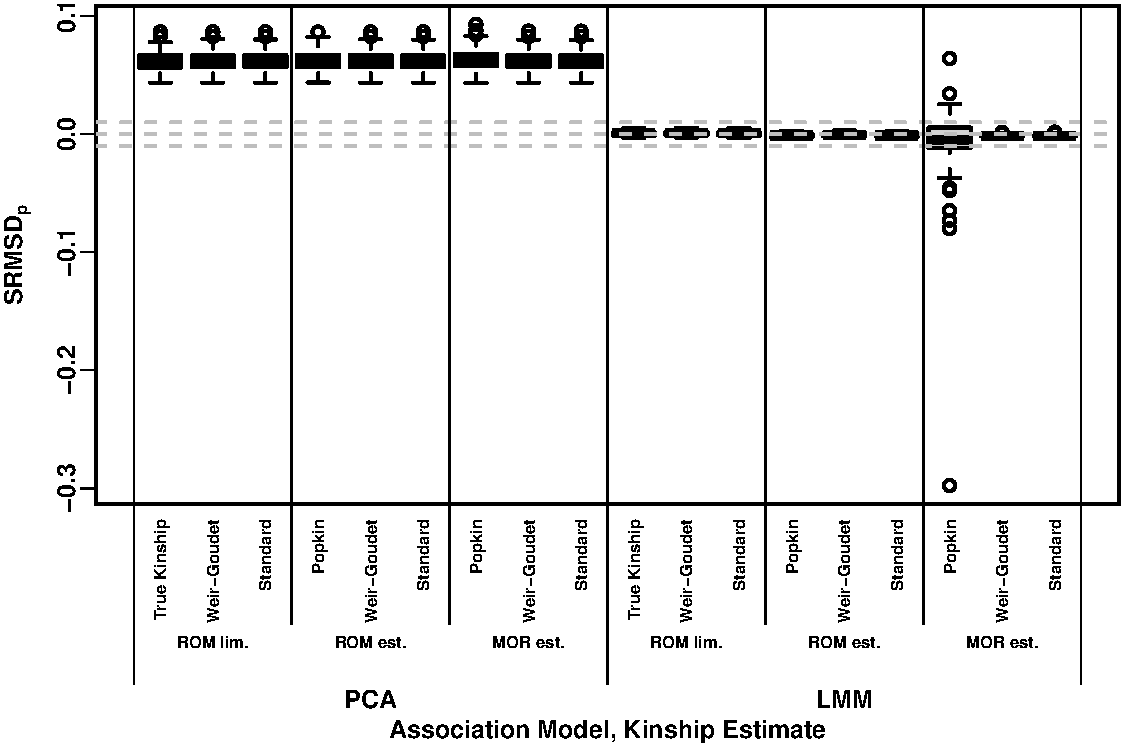
\includegraphics[width=\textwidth]{sim-admix-n1000-m100000-k3-f0.3-s0.5-mc100-h0.8-g20-fes/rmsd.pdf}
  \caption{
    {\bf Signed Root Mean Square Deviation of null p-values ($\rmsd$) for every combination of association model and kinship estimate on the admixed family simulation.}
    }
  \label{fig:rmsd_sim}
\end{figure}

\begin{figure}[hp!]
  \centering
  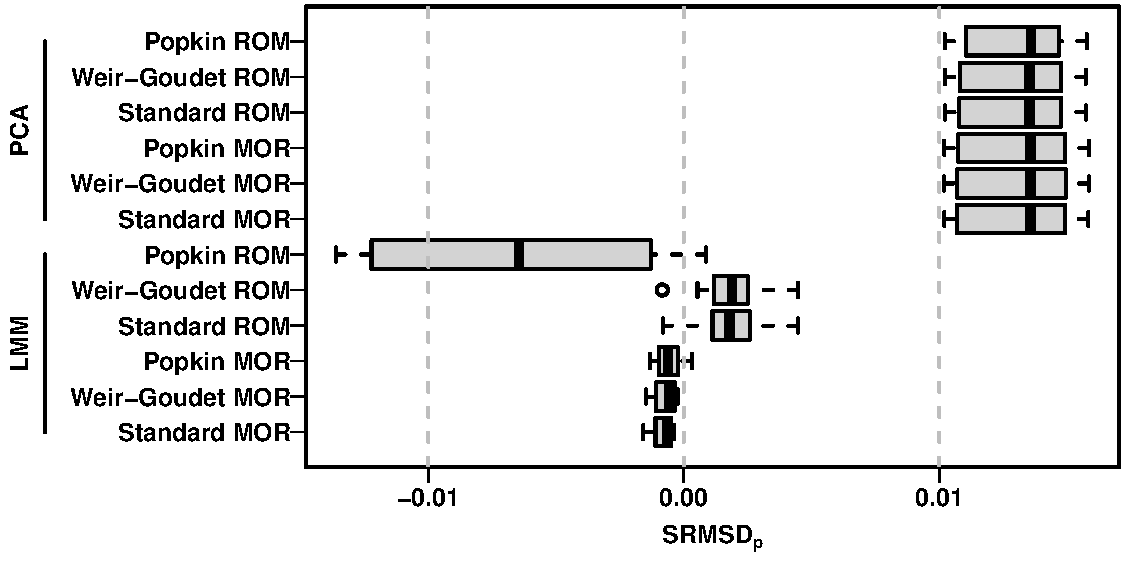
\includegraphics[width=\textwidth]{tgp-nygc-autosomes_ld_prune_1000kb_0.3_maf-0.01/rmsd.pdf}
  \caption{
    {\bf Signed Root Mean Square Deviation of null p-values ($\rmsd$) for every combination of association model and kinship estimate on 1000 Genomes.}
  }
  \label{fig:rmsd_real}
\end{figure}

\begin{figure}[hp!]
  \centering
  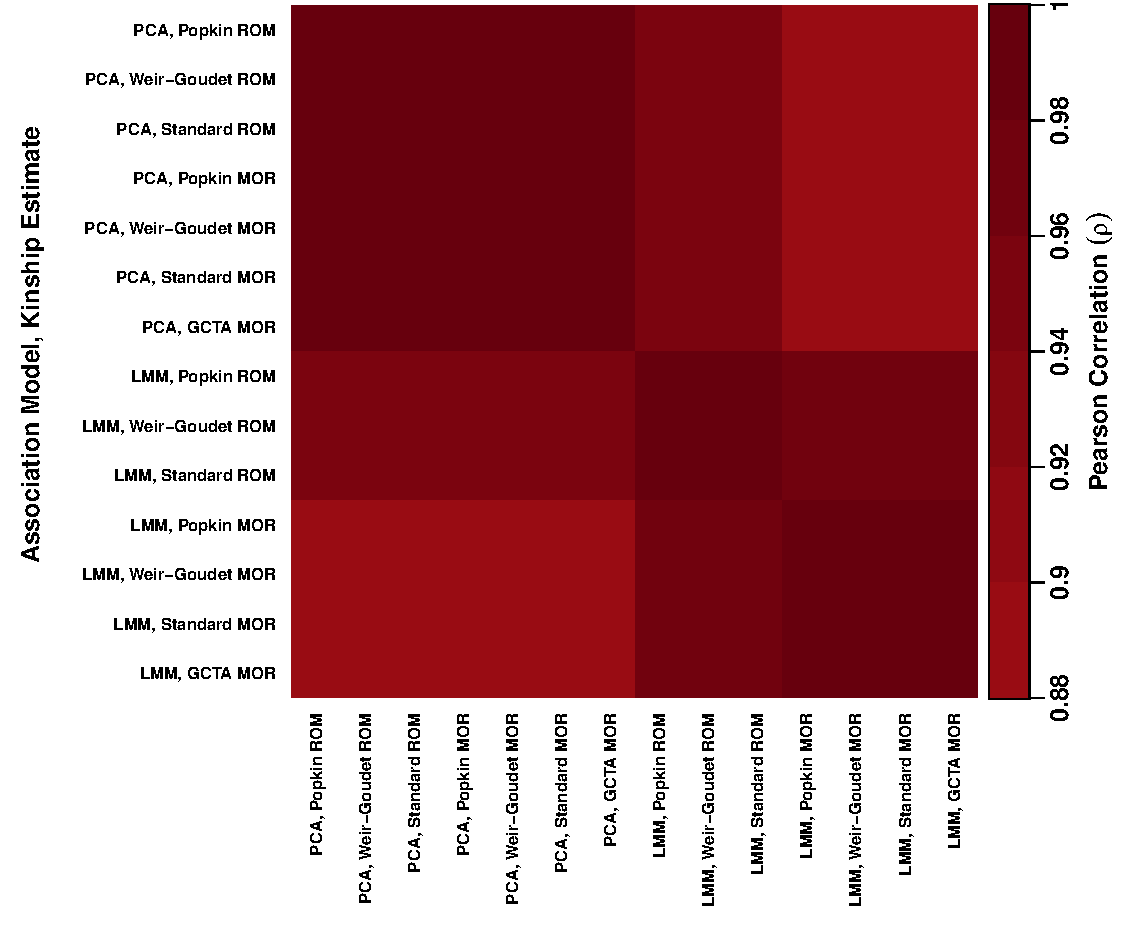
\includegraphics[width=\textwidth]{tgp-nygc-autosomes_ld_prune_1000kb_0.3_maf-0.01/pvals_cor.pdf}
  \caption{
    {\bf Correlation between p-values of different association models and kinship estimates on 1000 Genomes.}
    The association p-value vector (one value per tested locus) produced by each combination of association model (LMM vs PCA) and kinship matrix (x and y axes) was used to compute Pearson correlations (color).
    P-values between all kinship matrices or association model (PCA or LMM) are highly correlated (including biased and unbiased estimates), and often the maximum correlation of 1 is achieved.
  }
  \label{fig:pvals_cor_real}
\end{figure}

\end{document}
